\documentclass[twocolumn]{article}
\usepackage{graphicx} % Required for inserting images
\usepackage{listings} % Replacing minted with listings
\usepackage[margin=25mm]{geometry}
\usepackage[indent=0mm]{parskip}
\usepackage{braket}
\usepackage{amssymb}
\usepackage[math]{cellspace}
\usepackage{xcolor} % to access the named colour LightGray
\definecolor{LightGray}{gray}{0.9}
\usepackage[
backend=biber,
style=chem-acs,
sorting=none
]{biblatex}
\addbibresource{ref.bib}
\usepackage{lmodern}  % Latin Modern, a sharper font
\usepackage[T1]{fontenc}

\usepackage{listings}
\lstset{
    backgroundcolor=\color{LightGray},
    basicstyle=\ttfamily,
    breaklines=true,
    frame=single,
    language=Python,
    keywordstyle=\color{blue},
    commentstyle=\color{green!60!black},
    stringstyle=\color{red}
}

\title{Winter School Hückel Homework}
\author{Fernando Mata Rabadán}
\date{}
\makeindex
\begin{document}

\maketitle


\section{Theoretical background}
The focus of this homework is to write a program that is able to obtain the eigenvalues and eigenstates of the Hückel Hamiltonian in carbon chains and rings. The Hückel Hamiltonian allows calculating the energies of conjugated $\pi$-systems. 

Hückel theory is a useful framework to understand aromatic systems and is based in the following approximations:
\begin{equation}
    H_{rr}^{eff, \pi} = \alpha
\end{equation}
Where $\alpha$ is the Coulombic integral and is determined experimentally.\cite{bishop1993group} This term is associated with the stabilization resulting from the electron-nucleus interaction with respect to the free electron. To define the interaction of an electron with nearby atoms, another approximation is made: 
\begin{equation}
    H_{rs}^{eff, \pi} =
\begin{cases} 
\beta & \text{if $r$ and $s$ are connected} \\
0 & \text{if they are not}
\end{cases}
\end{equation}
Where $\beta$ is the resonance integral and also obtained experimentally.\cite{bishop1993group} Hückel theory considers that a bound electron interacts with neighbouring atoms only. This interaction produces a stabilizing effect on the electron and due to the approximation the effective Hamiltonian between atoms that are not connected is considered $0$. Finally, these parameters show a \(1/r^2\) dependence. This implies that a difference in atom size or interatomic distances will result in different stabilization. 

The nearest-neighbours interaction is reflected in the  construction of the Hamiltonian matrix. The Hückel Hamiltonian matrix is built with $\alpha$ as the diagonal terms and $\beta$ in the off-diagonal terms of interacting atoms. A simple example of pentane atoms would be: 
\begin{equation}
    \hat{H}_{\textrm{Hückel}}  =
    \begin{pmatrix}
        \alpha & \beta & 0 & 0 & 0 \\
        \beta & \alpha & \beta & 0 & 0 \\
        0 & \beta & \alpha & \beta & 0 \\
        0 & 0 & \beta & \alpha & \beta \\
        0 & 0 & 0 & \beta & \alpha \\
    \end{pmatrix}
\end{equation}
    
Where the first atom is connected to the second, the second to the third and so on. By diagonalizing this Hamiltonian, the energies and wave functions of the system are found:
\begin{equation}
    \hat{H}_{\textrm{Hückel}}\ket{\Psi_i}   =  E_{i}\ket{\Psi_i}
\end{equation}

The Hückel Hamiltonian can also be applied to rings. In this case, this can be done by including the matrix elements that connect the first and last atoms. In the case of cyclopentane it would be: 
\begin{equation}
    \hat{H}_{\textrm{Hückel}}  =
    \begin{pmatrix}
        \alpha & \beta & 0 & 0 & \beta \\
        \beta & \alpha & \beta & 0 & 0 \\
        0 & \beta & \alpha & \beta & 0 \\
        0 & 0 & \beta & \alpha & \beta \\
        \beta & 0 & 0 & \beta & \alpha \\
    \end{pmatrix}
\end{equation}

As the quantity of interest is the relative energy difference between states, it is possible to set $\alpha=0$, as this does not affect the relative energy of eigenvalues. When there are different types of atoms, the value of $\alpha$ will not be the same, and thus this must be reflected in the Hamiltonian matrix. An example of a chain of 5 alternating atoms would be:
\begin{equation}
    \hat{H}_{\textrm{Hückel}}  =
    \begin{pmatrix}
        \alpha & \beta & 0 & 0 & 0 \\
        \beta & \alpha'  & \beta & 0 & 0 \\
        0 & \beta & \alpha & \beta & 0 \\
        0 & 0 & \beta & \alpha'  & \beta \\
        0 & 0 & 0 & \beta & \alpha \\
    \end{pmatrix}
\end{equation}
Where $\alpha$ corresponds to the first atom type and $\alpha'$ to the second. Similarly, the value of $\beta$ depends on the interatomic distance.- Therefore, it is possible to express differences in bond lengths between atoms setting two different values of beta $\beta^+$ and $\beta^-$. In the case of pentadiene: 
\begin{equation}
    \hat{H}_{\textrm{Hückel}}  =
    \begin{pmatrix}
        \alpha & \beta^+ & 0 & 0 & 0 \\
        \beta^+ & \alpha & \beta^- & 0 & 0 \\
        0 & \beta^- & \alpha & \beta^+ & 0 \\
        0 & 0 & \beta^+ & \alpha & \beta^- \\
        0 & 0 & 0 & \beta^- & \alpha \\
    \end{pmatrix}
\end{equation}
Where  $\beta^+$ corresponds to a longer bond distance and $\beta^-$ to a shorter one. 

\section{Program review}
The initial intent was to write the program in FORTRAN, but due to problems with (probably) my compiler errors arose. When calling a matrix diagonalization using  lapack, the eigenvalues and eigenvectors were mismatched, rendering it impossible to order and plot the different states with the correct energies. Due to this, the program was rewritten in python, while maintaining the core functionality. While the code is written with a class structure, for clarity the code shown here is a simplification. 

\subsection{Code analysis}
The code is divided in two main parts: a class \texttt{Chain} that handles all the properties related to the Hückel Hamiltonian and a function \texttt{run\_calculation} that handles the general flow of a calculation. The advantage of working with a class is that it is possible to create various instances of these chains or rings and compare results and plot them easily and directly. 

\subsubsection{The \texttt{Chain} class}
The \texttt{Chain} class compacts both the calculation and plotting of the eigenvalues and eigenvectors of the system Hamiltonian. The Chain class has the following methods that allow the modification of internal variables:
\begin{lstlisting}
    Chain.close_ring() # sets the internal variable Chain._ring to True
    Chain.open_ring() # sets the internal variable Chain._ring to False
    Chain.set_beta_minus() #  sets the internal variable Chain._beta_minus to False
    Chain.set_alpha_prime() # sets the internal variable Chain._alpha_prime to False
\end{lstlisting} 
These internal variables are accessed when building the Hamiltonian, modifying the different possible cases. 

\paragraph{\texttt{Chain.huckel\_matrix}:}
The Hamiltonian is stored as a property. The function considers different cases in the following way:

\begin{itemize}
    \item Alternating bond distances: in order to simulate different bond distances, the value of the \(\beta\) value is modified in the Hamiltonian. In this case, the value of \(\beta^+\) is set always to \(-1\) while the value of \(\beta^-\) can be set to a different value with \texttt{Chain.set\_beta\_minus}. To take into account this alternation of betas, the \texttt{Chain.huckel\_matrix} modifies the Hamiltonian matrix with:
\begin{lstlisting}[backgroundcolor=\color{LightGray}]
    for i in range(n_atoms - 1):
        if i % 2 == 0:
            huckel_matrix[i + 1, i] = -1 
            huckel_matrix[i, i + 1] = -1
        else:
            huckel_matrix[i + 1, i] = beta_minus
            huckel_matrix[i, i + 1] = beta_minus
\end{lstlisting} 
    It iterates over the matrix and changes the value of beta when the index is odd. 
    \item Alternating atoms: Similarly to alternating distances, to take into account alternating atoms, it is possible to set a different value to the $\alpha$ value of the diagonal matrix elements with \texttt{Chain.set\_alpha\_prime}. As with the previous property, only the possibility of modifying one of the two $\alpha$ values was considered, and this is reflected in the Hamiltonian matrix with:
\begin{lstlisting}[backgroundcolor=\color{LightGray}]
    for i in range(n_atoms):
        if i % 2 == 0:
            huckel_matrix[i, i] = 0
            huckel_matrix[i, i] = 0
        else:
            huckel_matrix[i, i] = alpha_prime
            huckel_matrix[i, i] = alpha_prime
\end{lstlisting} 
    
    \item Rings: Rings are built by connecting the first and last atoms of a given chain. This is done explicitly as:
\begin{lstlisting}[backgroundcolor=\color{LightGray}]
    if ring == True:
        huckel_matrix[0, n_atoms - 1] = -1
        huckel_matrix[n_atoms - 1, 0] = -1
\end{lstlisting} 
The condition of the object being a ring is checked and if so the last values of the first row and column are adjusted accordingly. 
        
\end{itemize}

\paragraph{\texttt{Chain.eigen}:} Once the Hamiltonian matrix is built, it can be diagonalized to obtain the eigenvalues and eigenvectors. The Chain.eigen stores as a property the eigenvalues and eigenvectors and calculates it via: 
\begin{lstlisting}[backgroundcolor=\color{LightGray}]
    def eigen():
        eigenvalues, eigenvectors = np.linalg.eig(huckel_matrix)
        
        # Sort eigenvalues and eigenvectors
        idx = np.argsort(eigenvalues) # returns the array with sorted indexes
        sorted_eigenvalues = eigenvalues[idx]
        sorted_eigenvectors = eigenvectors[:, idx]

        eigenvalues = sorted_eigenvalues
        eigenvectors = sorted_eigenvectors

        return sorted_eigenvalues, sorted_eigenvectors
\end{lstlisting} 
The Hückel matrix is diagonalized using the numpy \texttt{linalg.eig} function. Then the pairs of eigenvalues and eigenvectors are sorted to return them in ascending order. 

Finally, the \texttt{Chain} class has two plotting functions:
\begin{lstlisting}[backgroundcolor=\color{LightGray}]
    Chain.plot_eigenvalues() # plots the eigenvalues of the Huckel Hamiltonian
    Chain.plot_eigenvectors() # plots the eigenvectors of the Huckel Hamiltonian
\end{lstlisting} 

\subsubsection{The \texttt{run\_calculation} Function and input handling}
The general scheme of any calculation using the program would be:
\begin{enumerate}
    \item Read the input.
    \item Modify properties accordingly to the input.
    \item Build and diagonalize the Hückel Hamiltonian.
    \item Return the results in a log file and the eigenvalues and eigenvectors in different files for external plotting.
\end{enumerate}

This workflow is managed by the \texttt{run\_calculation} function. The input file is read with:

\begin{lstlisting}[backgroundcolor=\color{LightGray}]
def run_calculation(input_filename, output_filename):
    content = load_input(input_filename)

    if content is None:
        return

    keyval_pairs = [ 
        tuple(line.replace('=', ' ').strip().split()[:2])
        for line in content 
        if len(line.replace('=', ' ').strip().split()) >= 2
    ]

    cont = dict(keyval_pairs)

    if 'n_atoms' not in cont.keys():
        raise ValueError('Definition of number of atoms is mandatory')
    
\end{lstlisting} 

The previous code reads all the content in the input file and generates a dictionary of property-value pairs. Therefore, the input keywords can be easily accessed. This way, it is possible to build the \texttt{Chain} object with the correct properties. Also, an error is raised if there is no information of the number of atoms of the system. Then the \texttt{Chain} object is created, and the properties modified with:

\begin{lstlisting}[backgroundcolor=\color{LightGray}]
    c = Chain(n_atoms=int(cont['n_atoms']))

    if 'ring' in cont.keys():
        if cont['ring'] == 'True':
            c.close_ring()

    if 'alternate_alpha' in cont.keys():
        alt_alpha = float(cont['alternate_alpha'])
        c.set_alpha_prime(alt_alpha)

    if 'alternate_beta' in cont.keys():
        alt_beta = float(cont['alternate_beta'])
        c.set_beta_minus(alt_beta)
\end{lstlisting} 

Finally, the eigenvalues and eigenvectors are calculated with:
\begin{lstlisting}[backgroundcolor=\color{LightGray}]
        eigenval, eigenvec = c.eigen    
\end{lstlisting} 

And the results written in the corresponding files.

In order to run the program from the terminal line, the \texttt{sys} module is imported, which allows reading the command line arguments. An error is raised if no input file is provided. 

\subsection{Usage and examples}
The program can be run from the command line by:
\begin{lstlisting}[backgroundcolor=\color{LightGray}]
    python3 huckel.py input_file output_file
\end{lstlisting} 
Where the specification of the output file is optional. A built-in help message is prompted in case of error. The input file should contain a list of keywords:

\begin{lstlisting}[backgroundcolor=\color{LightGray}]
    n_atoms = 100
\end{lstlisting} 
And optional values such as cyclization, distance alternation and atom alternation can be set with:
\begin{lstlisting}[backgroundcolor=\color{LightGray}]
    ring = False
    alternate_alpha = 0.0
    alternate_beta = -1.0
\end{lstlisting} 
The input is case-sensitive, and the program will not run if keywords are not exactly the same. Also, the values True and False must have the first capital letter.

An advantage of working with classes is that the simplicity to calculate and plot different chains and cases, for example to compare the open chain and ring cases it would be:
\begin{lstlisting}[backgroundcolor=\color{LightGray}]
    from huckel import Chain
    a = Chain(10)
    b = Chain(10)
    
    b.close_ring()
    
    a.plot_eigenvalues()
    b.plot_eigenvalues()
\end{lstlisting} 
And the same with the  \texttt{set\_alpha\_prime()} and \texttt{set\_beta\_minus()} methods. All the scripts to obtain the figures in the next section can be found in the \texttt{plots/} directory. 

\section{Results}
Having defined the whole framework in the previous class, it is possible to calculate the eigenvalues and eigenvectors of different systems. The systems that are simulated are the conjugated $\pi$-systems of chains and rings. 

\subsection{Chain vs Ring}
First, the eigenvalues and eigenvectors of both a chain and a ring of 10 atoms were calculated. The results are shown in Figure \ref{fig:chain_ring}. It is possible to appreciate a clear difference between the two cases. The chain system does not present repeated eigenvalues, while the ring presents two-fold degeneracy. This is consistent with the expected results of Hückel MO theory, where there are degenerated states two by two in rings. 

\begin{figure}[ht]
    \centering
    \begin{minipage}{0.47\textwidth}
        \centering
        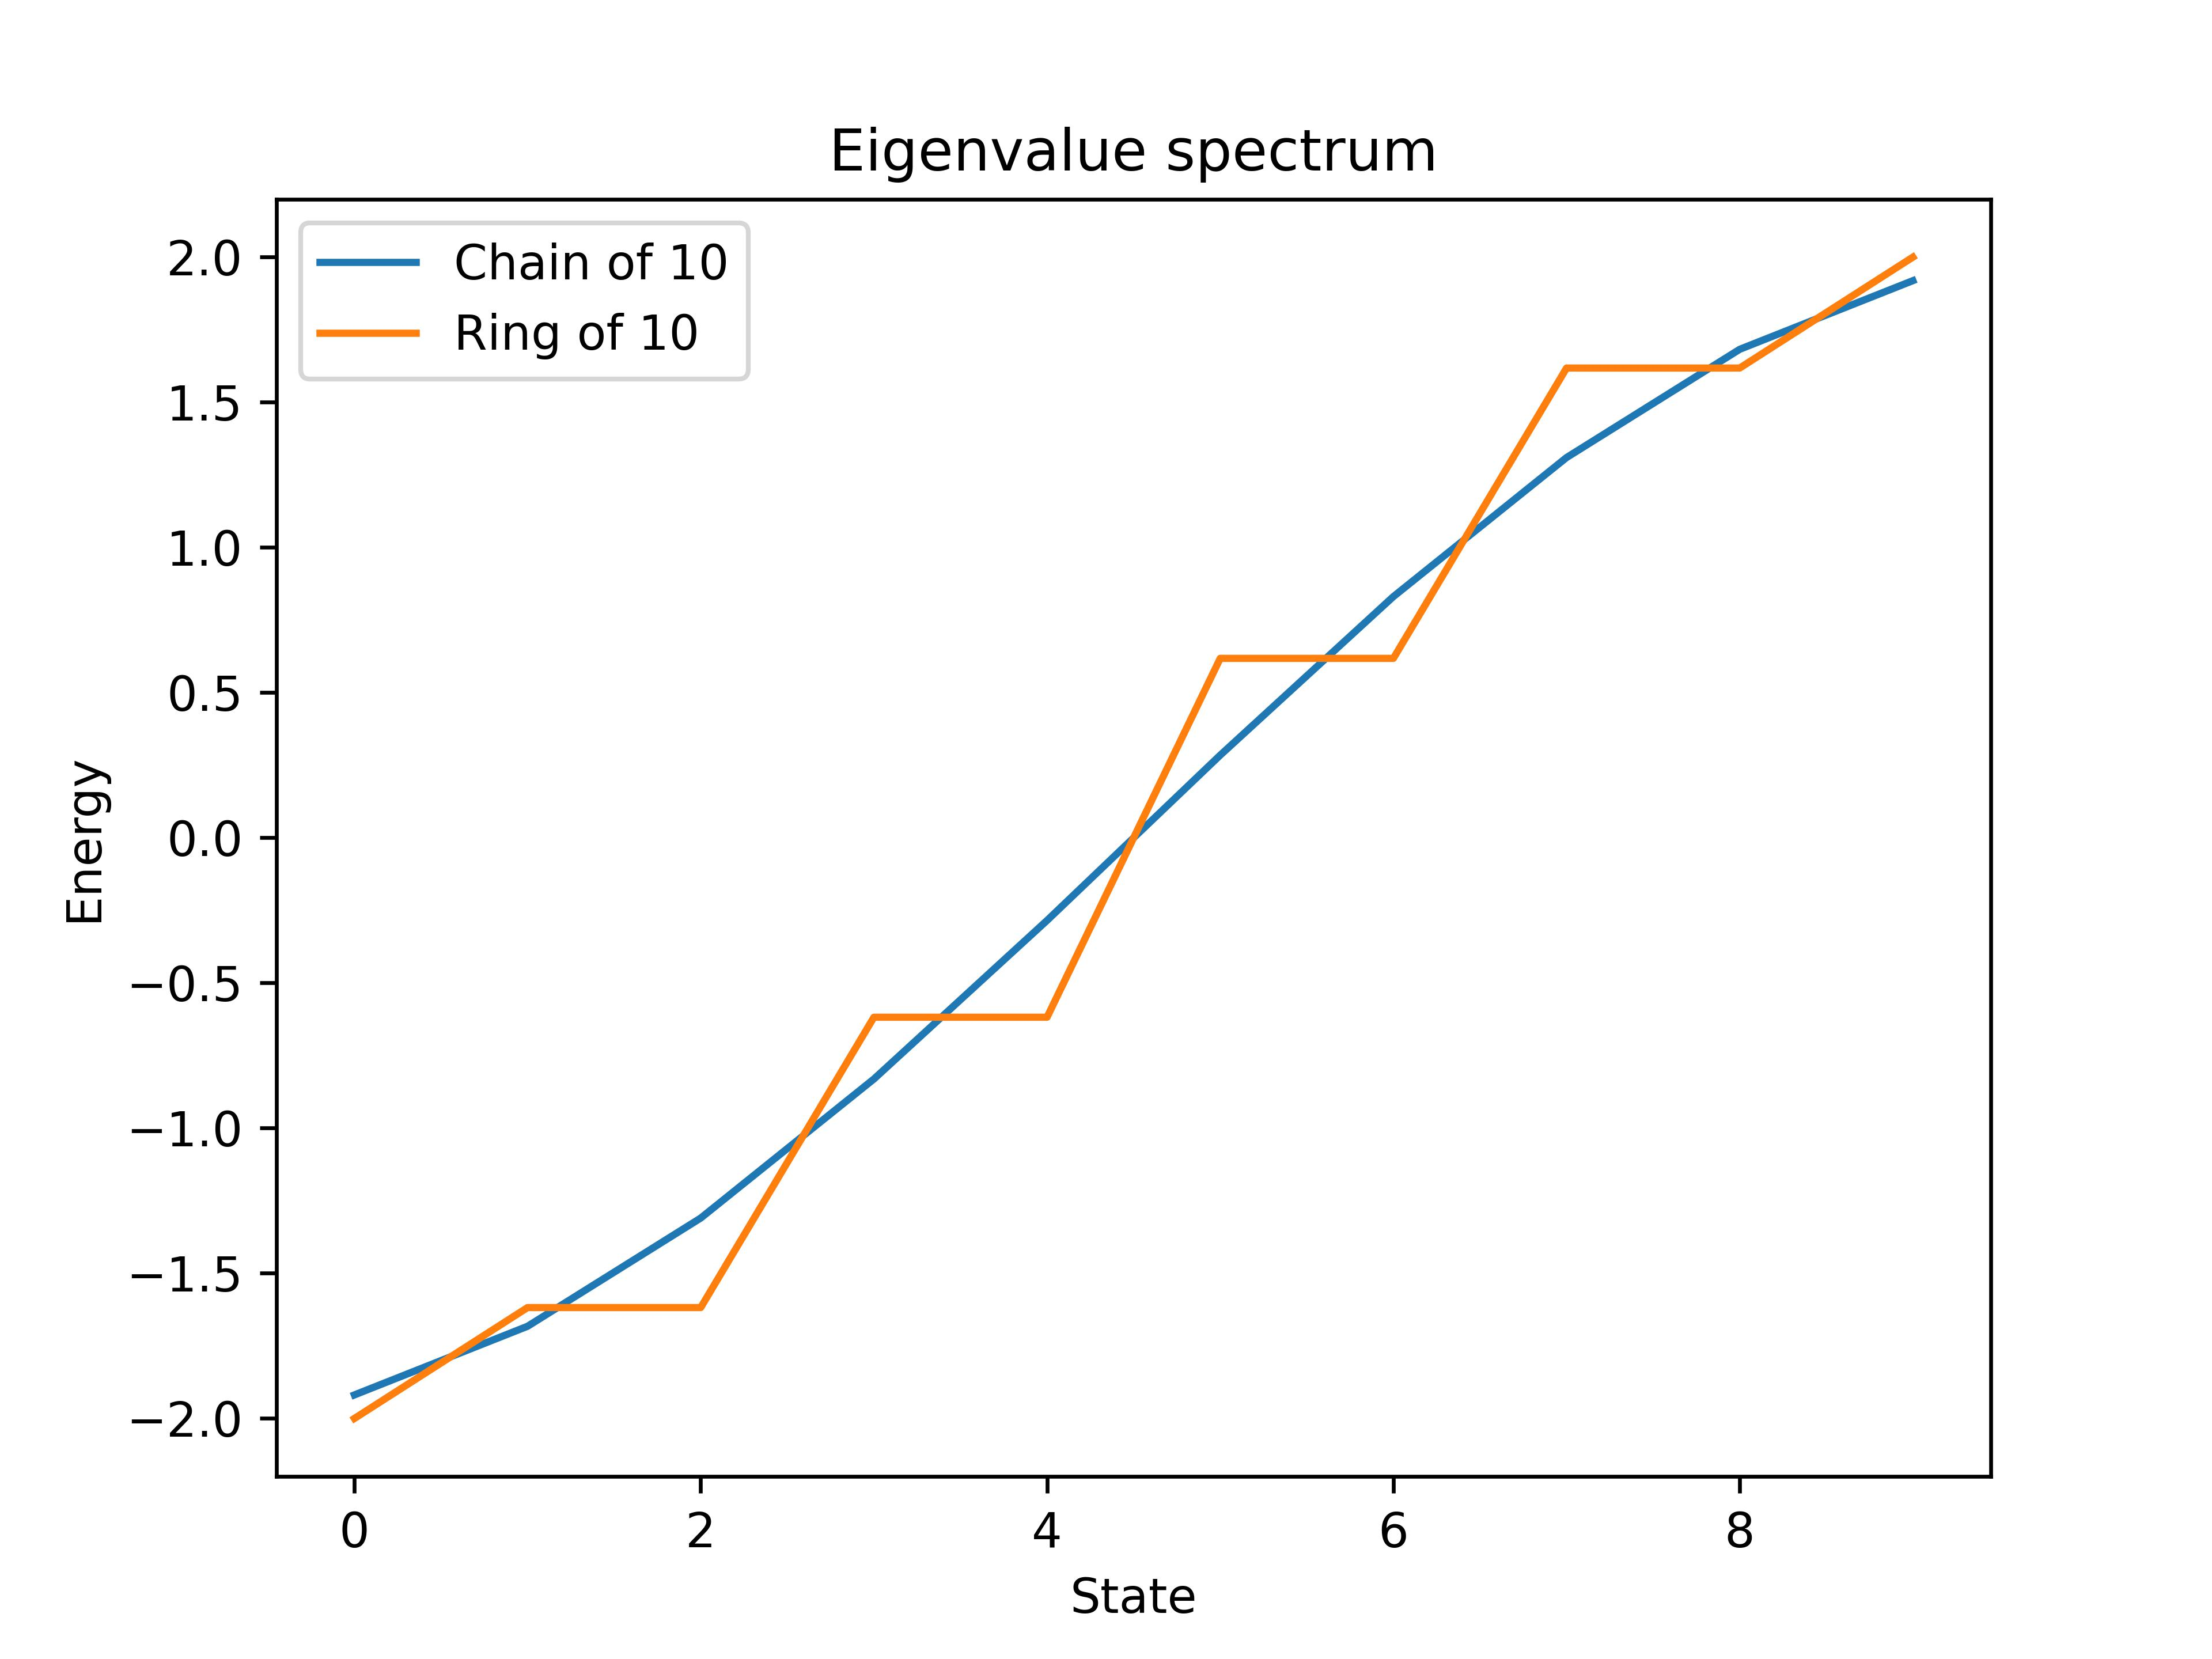
\includegraphics[width=\textwidth]{Figures/chain_vs_ring.jpg}
        \caption{Comparison of eigenvalues for a chain and a ring of 10 atoms.}
        \label{fig:chain_ring}
    \end{minipage}
    \hfill
    \begin{minipage}{0.47\textwidth}
        \centering
        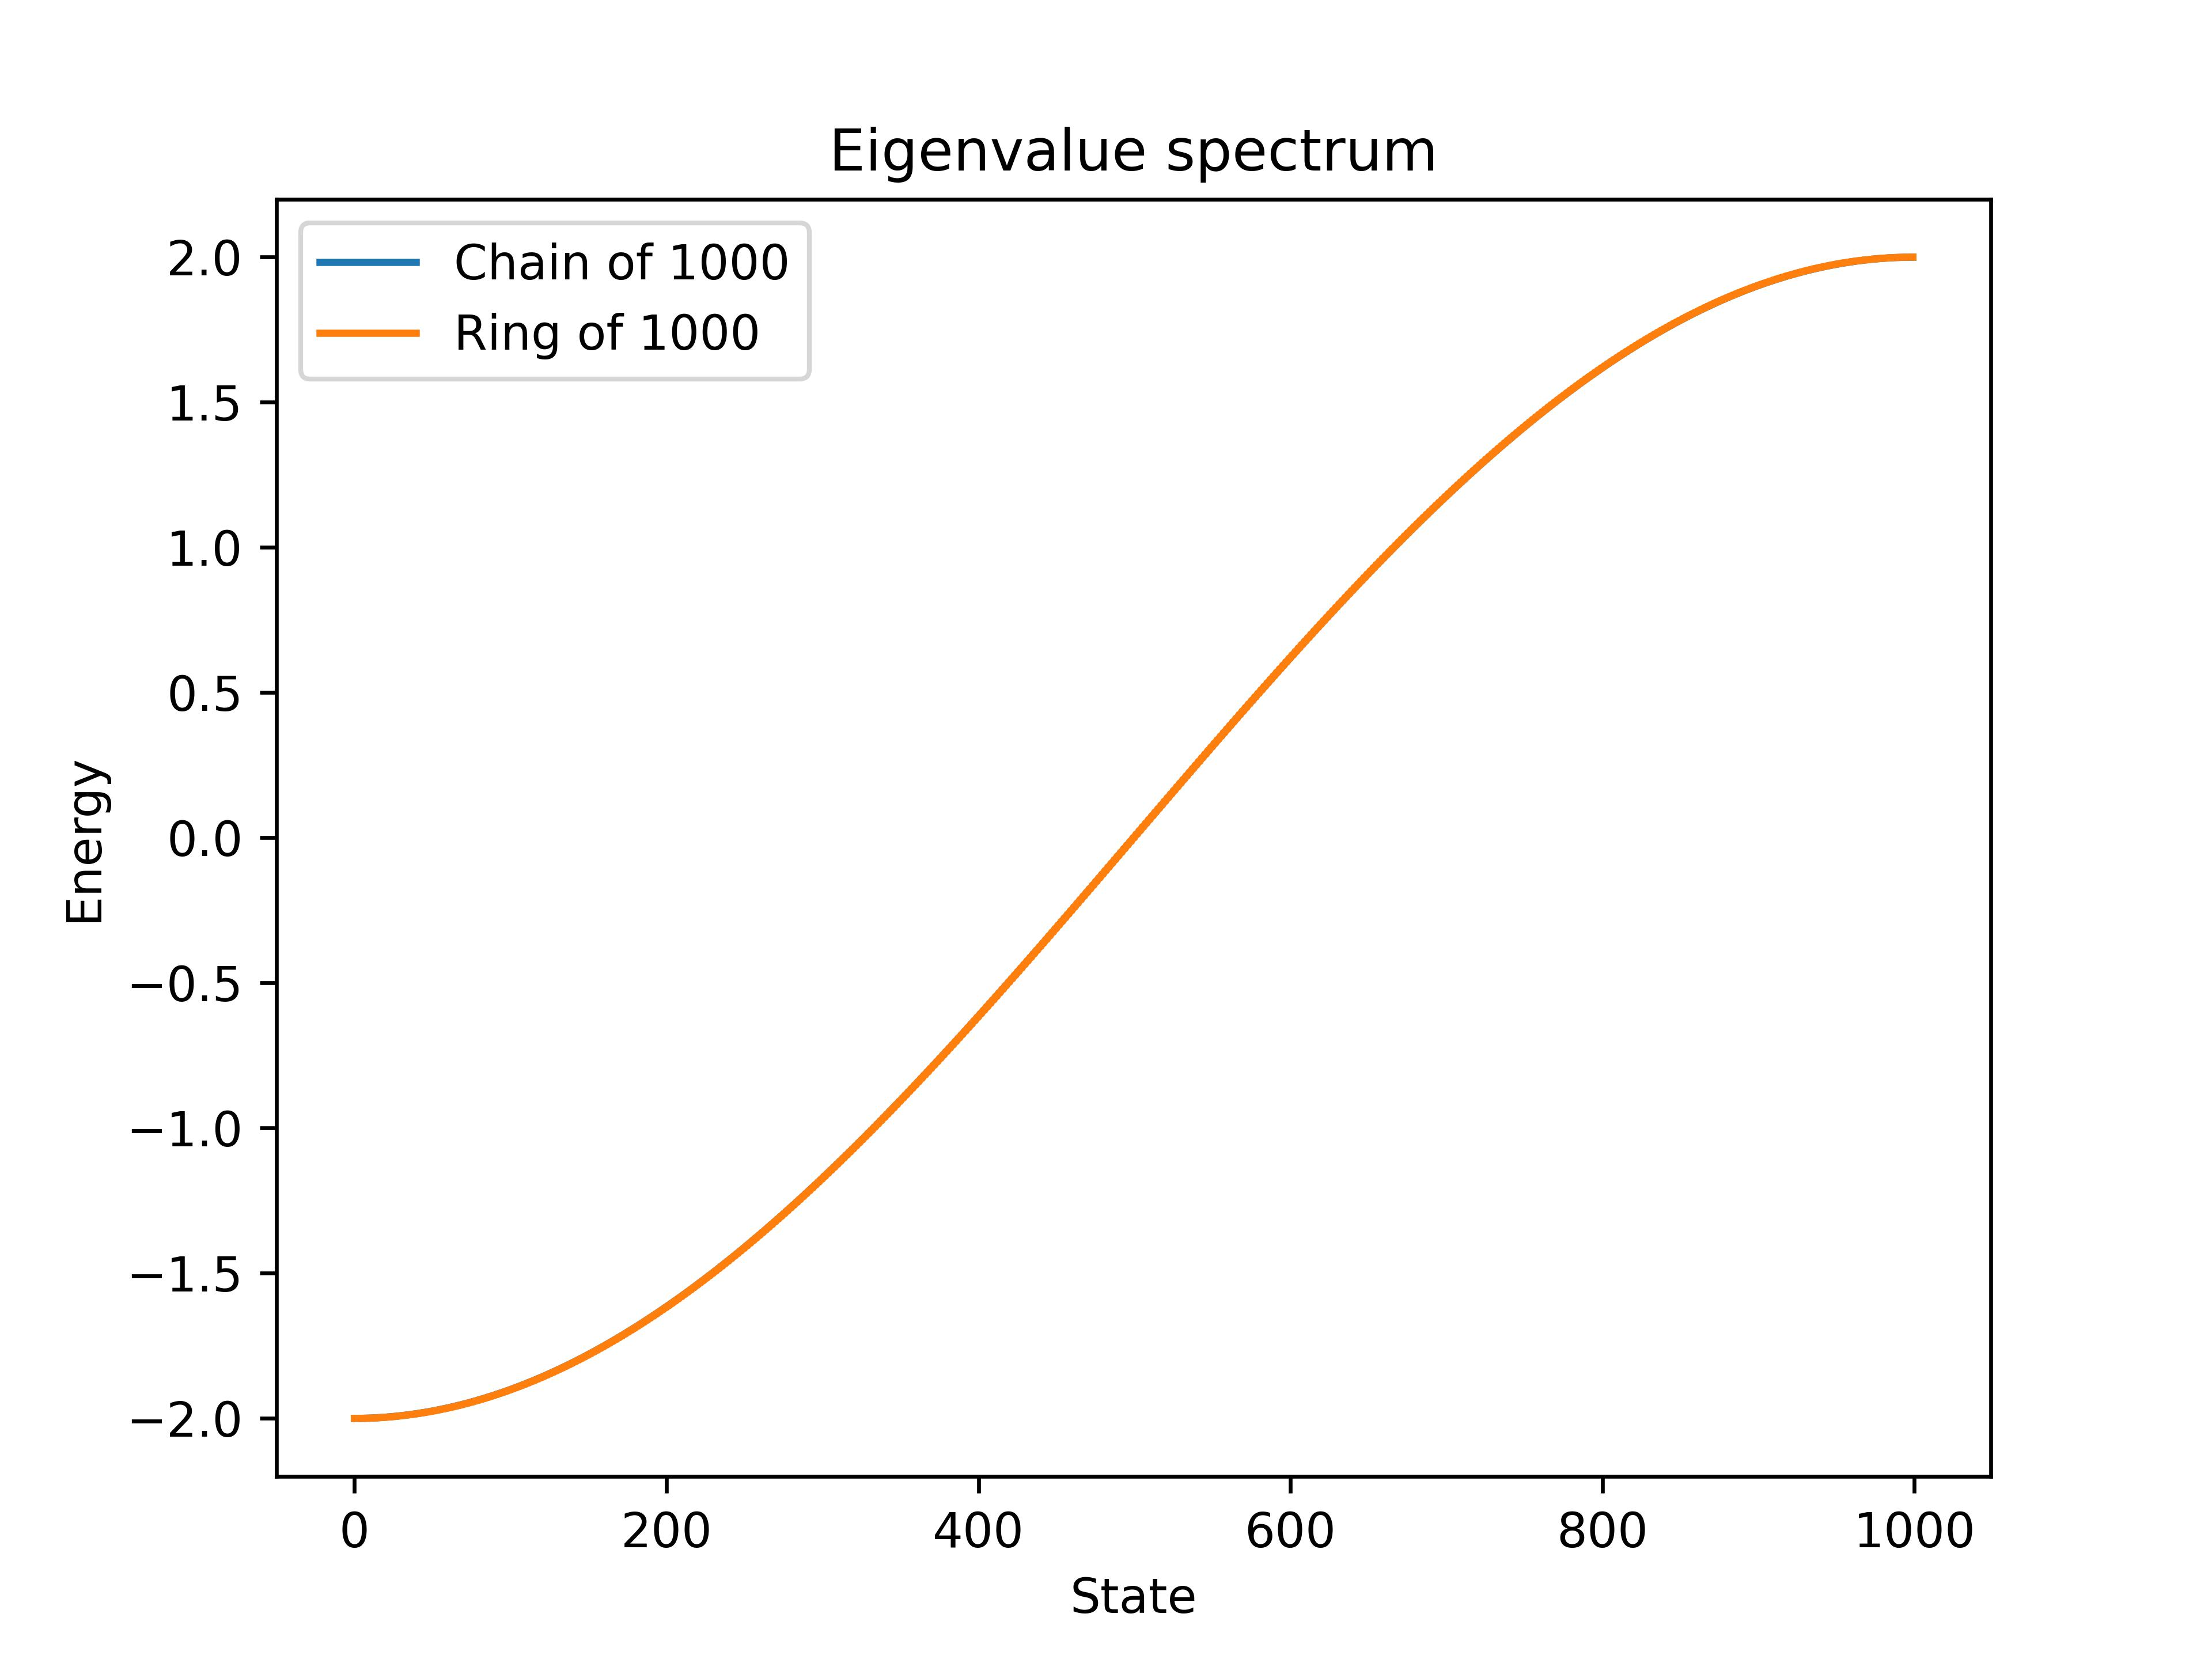
\includegraphics[width=\textwidth]{Figures/convergence_limit.jpg}
        \caption{Comparison of eigenvalues for a chain and a ring of 1000 atoms.}
        \label{fig:chain_vs_ring_infinite}
    \end{minipage}
\end{figure}

Eigenvectors of the first states are shown in Figures \ref{fig:chain_eigenvectors} and \ref{fig:ring_eigenvectors}. There is a significant difference in the eigenvector spectrum. While the wave function of the chain in the ground state is localized in the central atoms like a particle in a box, the ring's wave function is delocalized over all the atoms. This is a consequence of the periodic boundary conditions (PBC) introduced. In the ring, electron movement can be looped, resulting in a delocalized state.

The wave function of excited states is also different. In the case of the chain, the wave function behaves as a particle in a box, presenting a number of nodes in the wave function corresponding to the excited state. In contrast, the ring presents a slightly different behaviour. Excepting the ground state, the $2n$ and $2n+1$ states present the same eigenfunction, but shifted. Due to the PBC imposed, both wave functions behave similarly, which results in the eigenvalue degeneracy. In the case of the ring, the number of nodes of will be $2n$ for that pair of eigenfunctions. 

\begin{figure}[ht]
    \centering
    \begin{minipage}{0.45\textwidth}
        \centering
        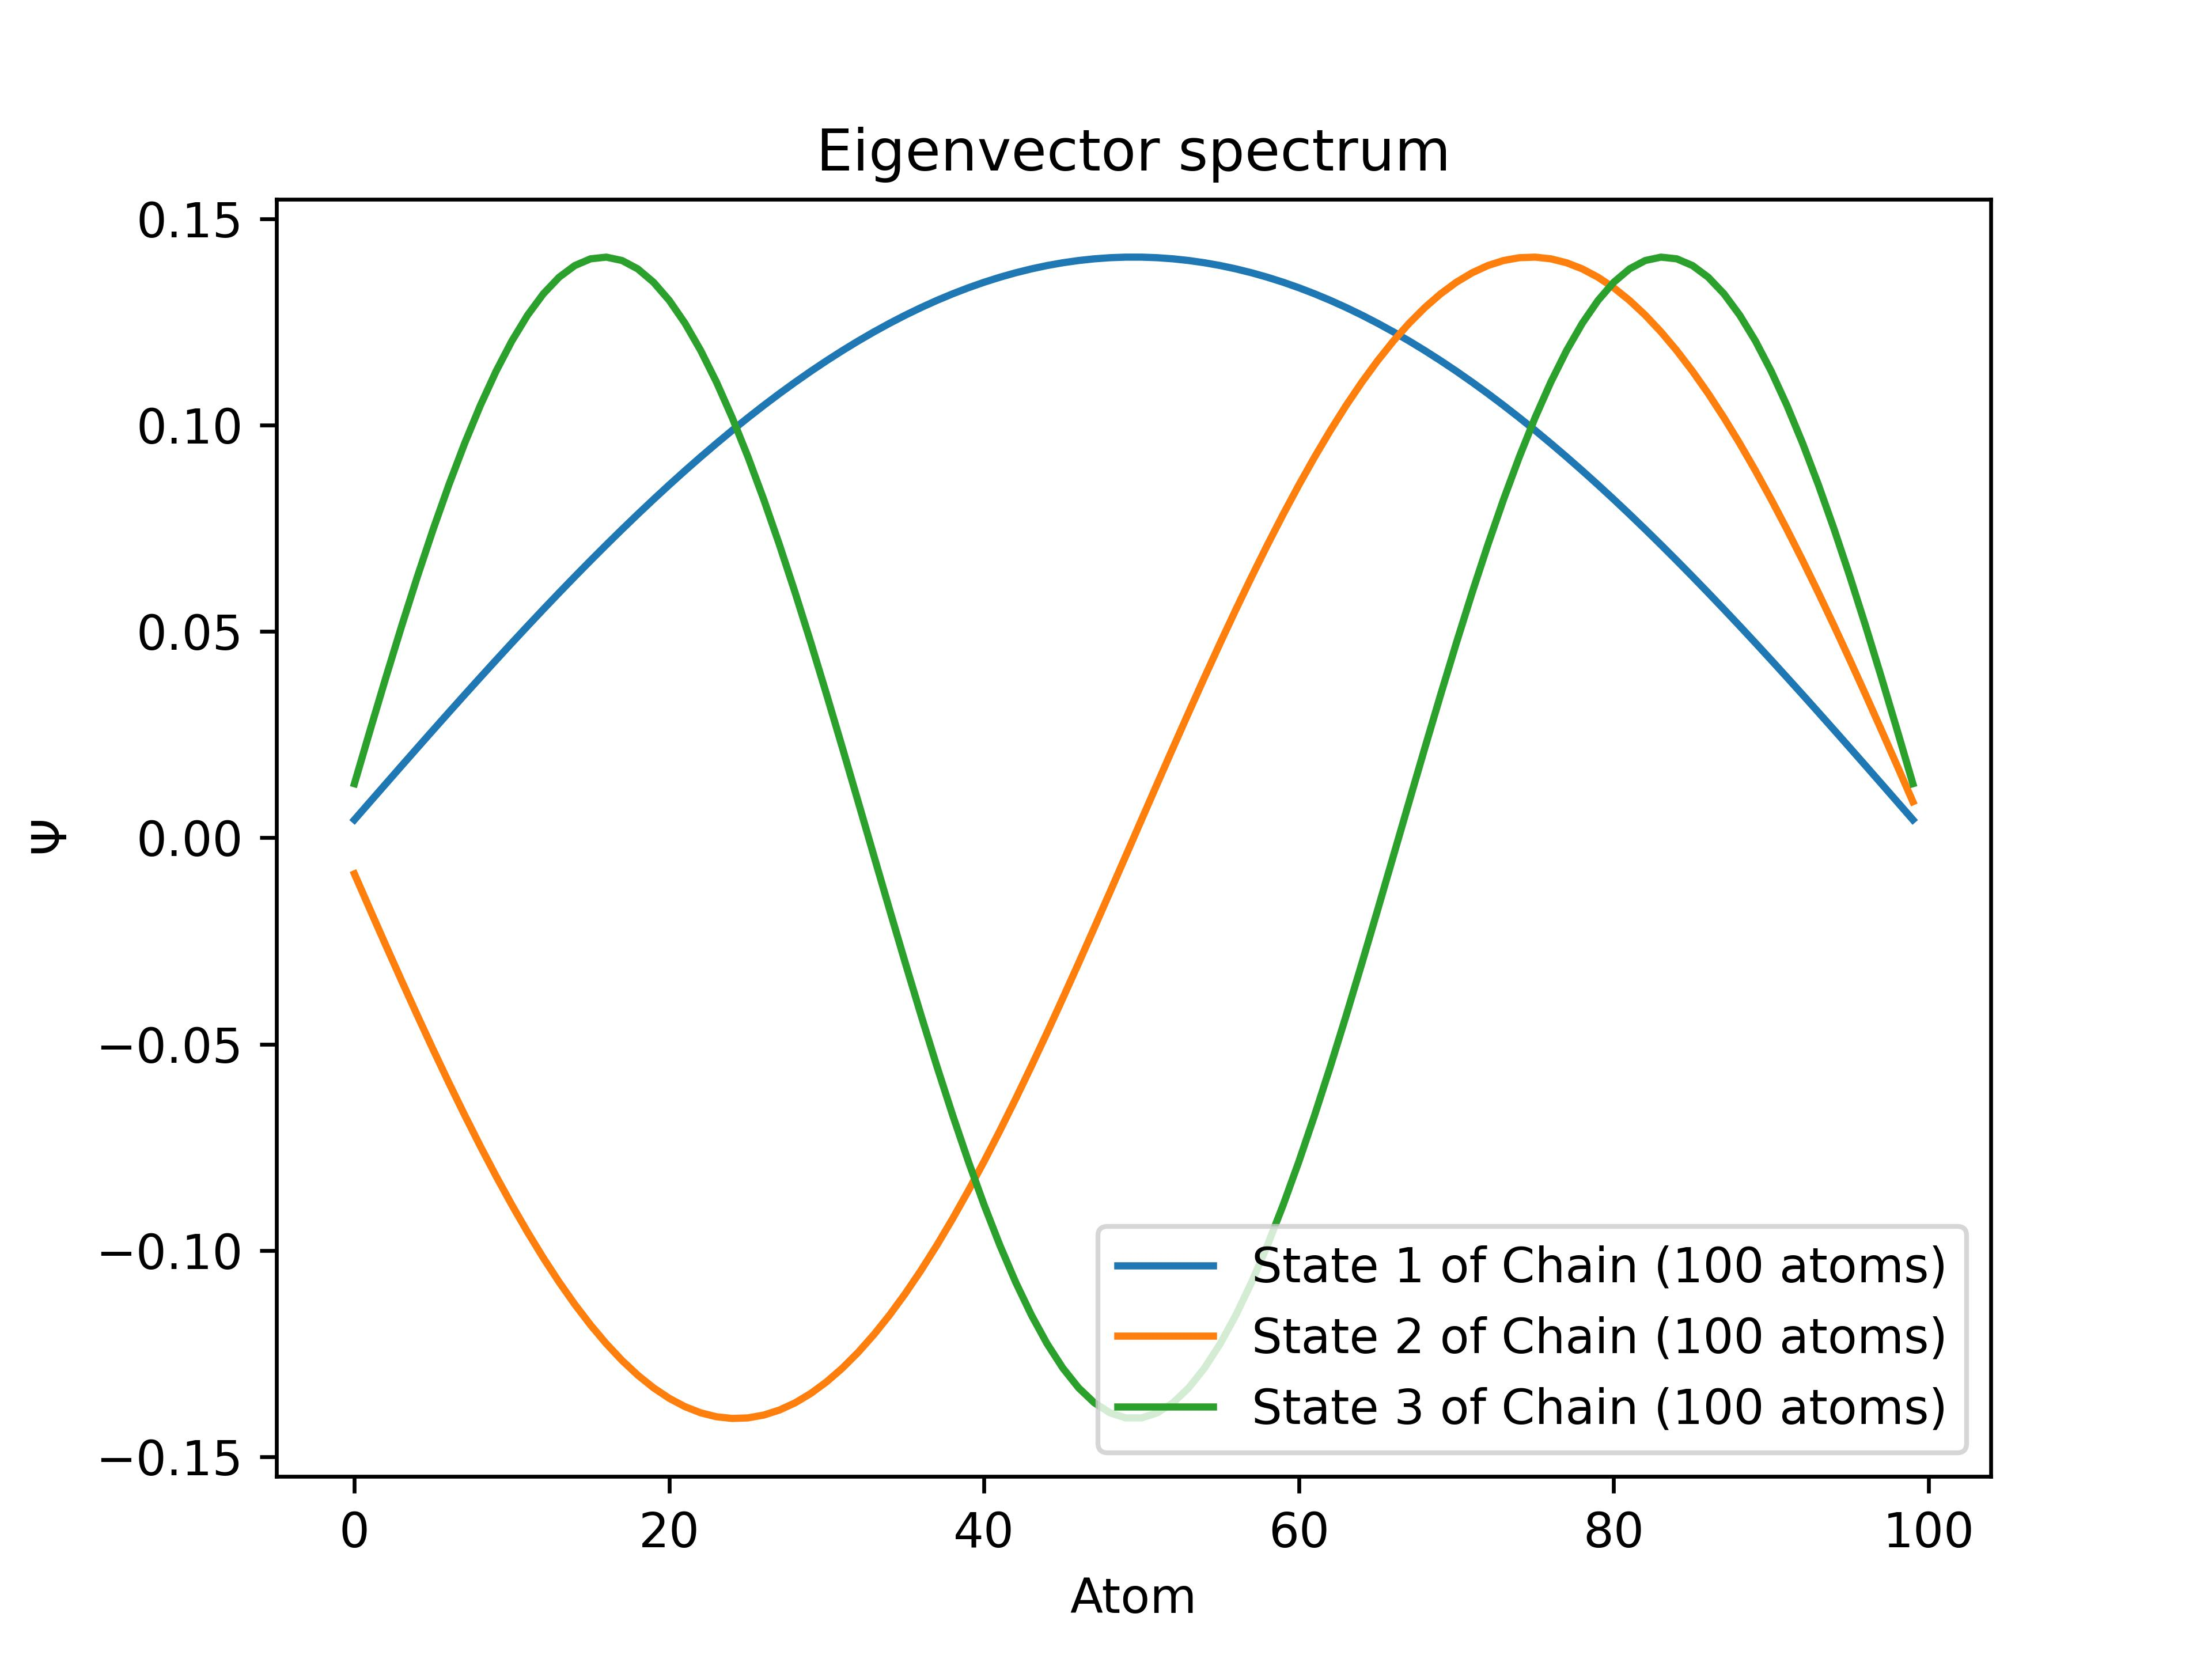
\includegraphics[width=\textwidth]{Figures/chain_eigenvectors.jpg}
        \caption{Eigenvectors for a chain of 10 atoms.}
        \label{fig:chain_eigenvectors}
    \end{minipage}
    \hfill
    \begin{minipage}{0.45\textwidth}
        \centering
        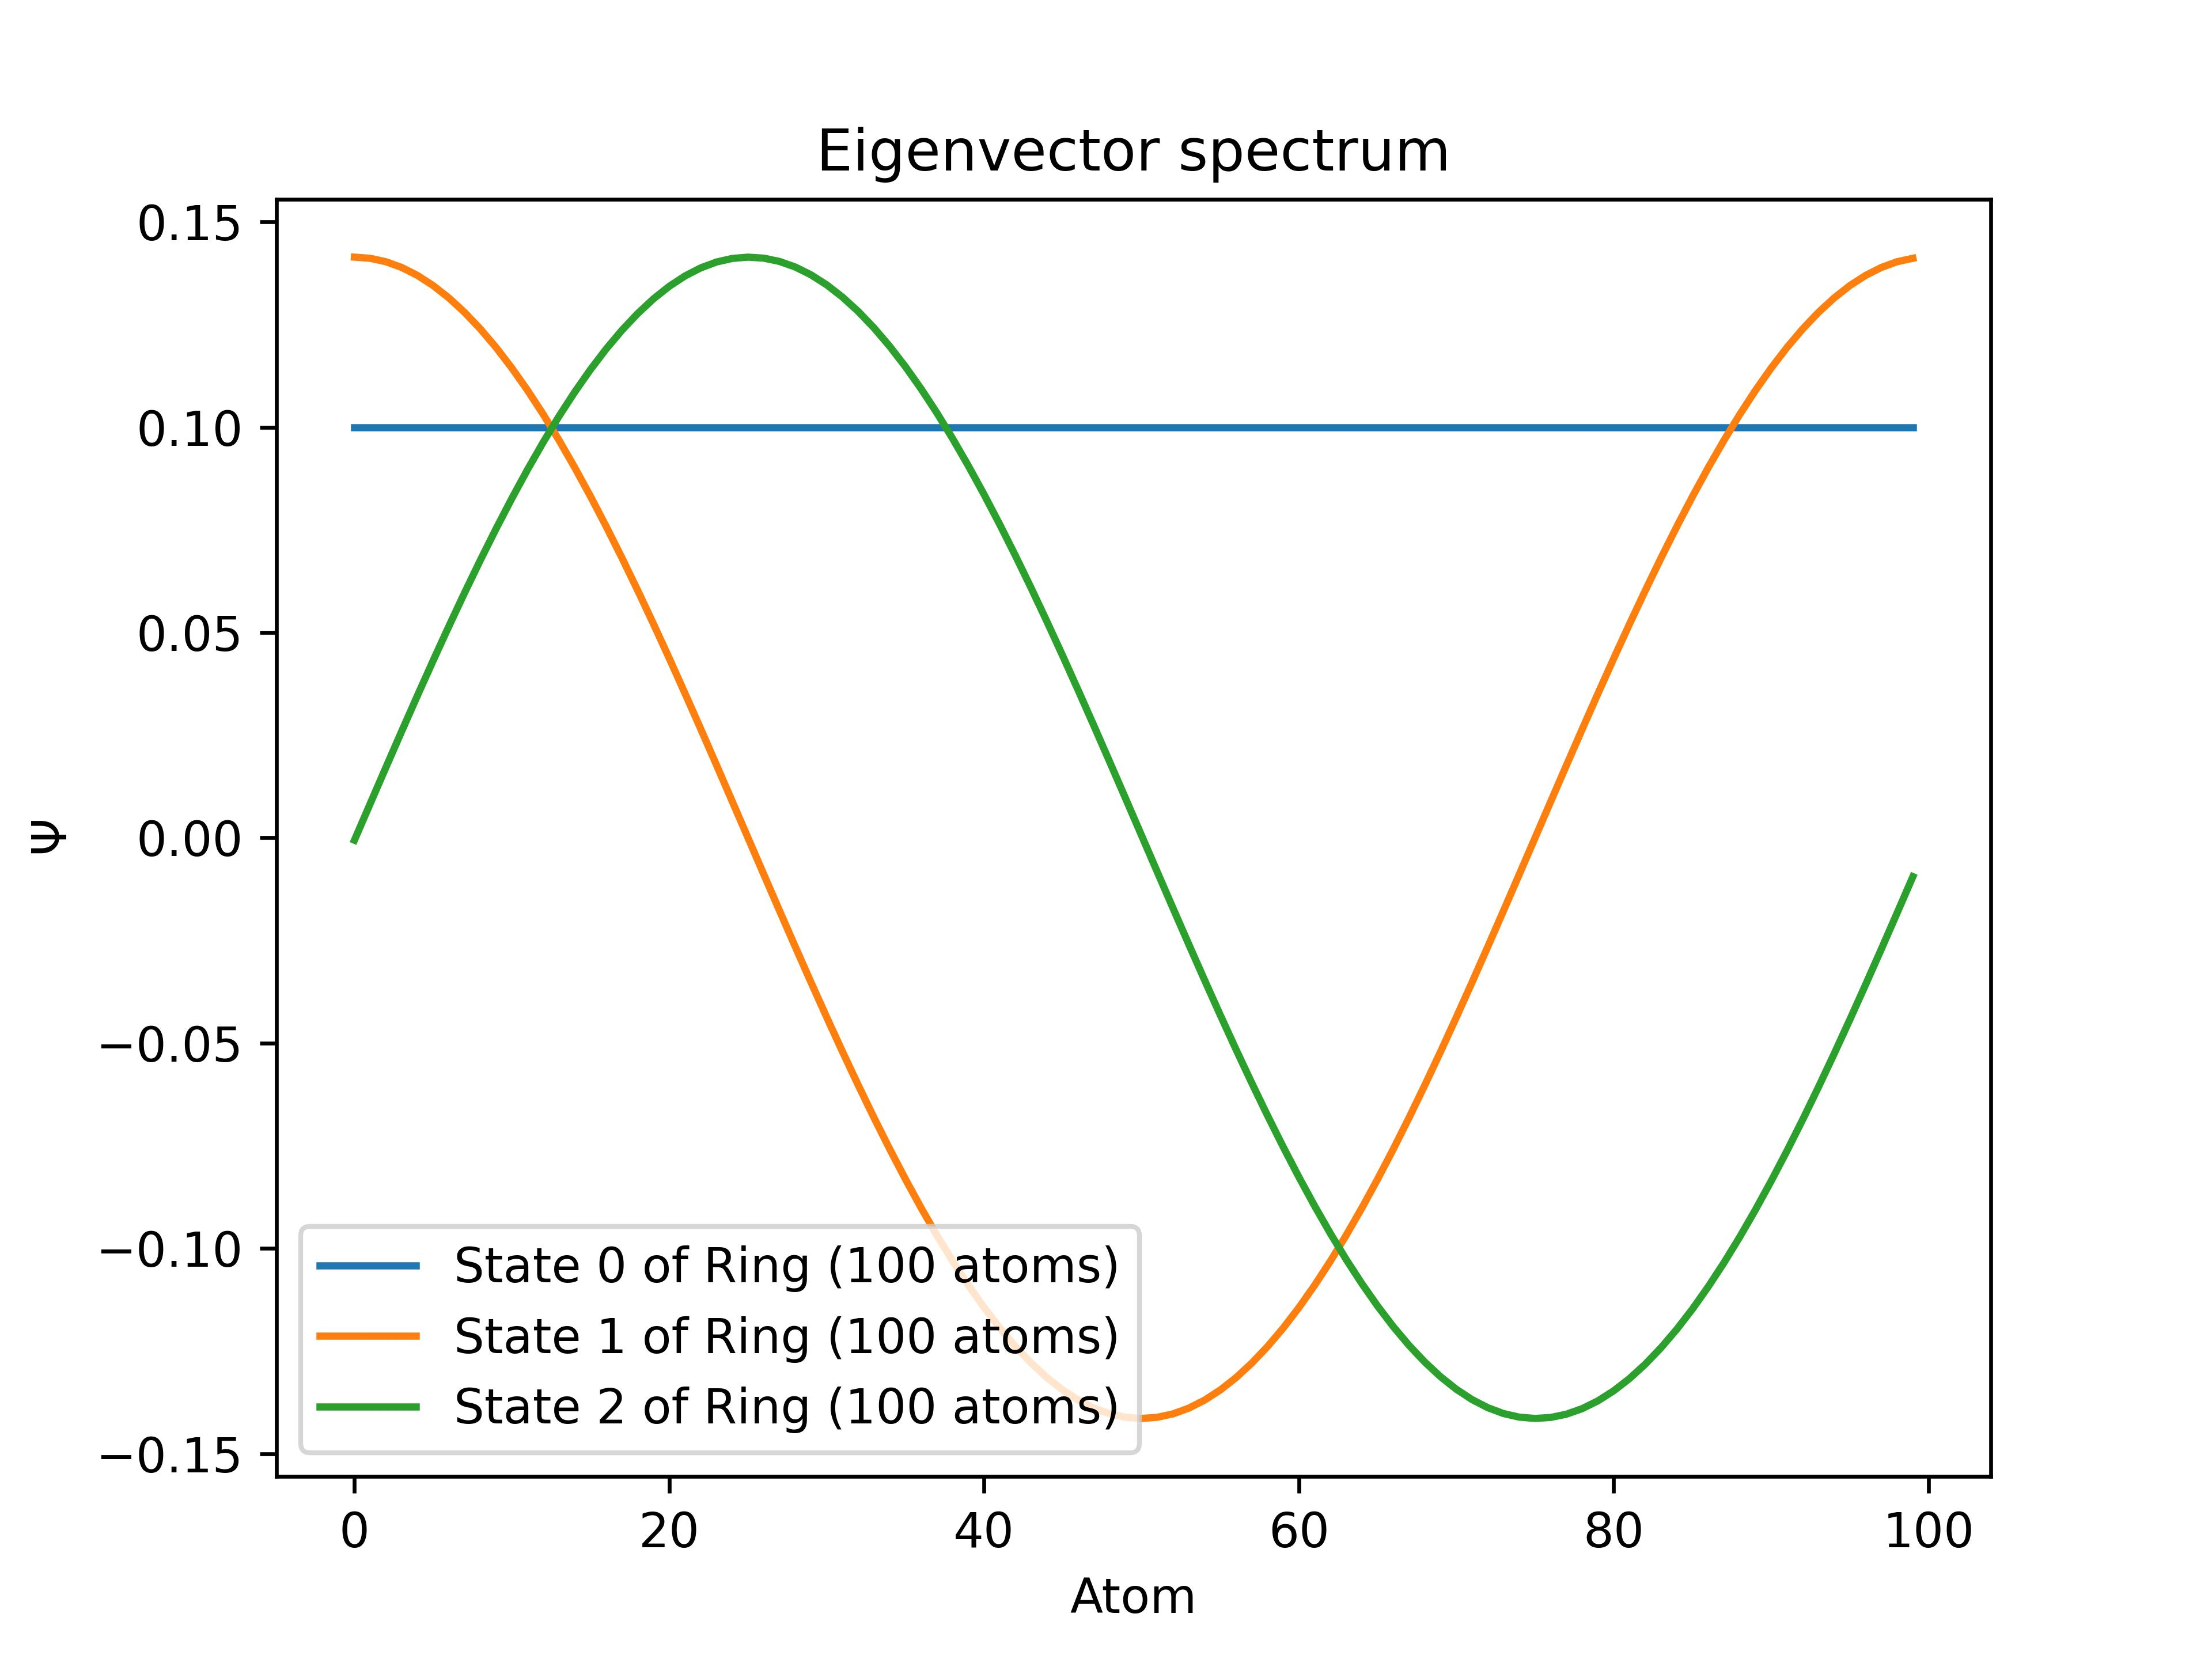
\includegraphics[width=\textwidth]{Figures/ring_eigenvectors.jpg}
        \caption{Eigenvectors for a ring of 10 atoms.}
        \label{fig:ring_eigenvectors}
    \end{minipage}
\end{figure}

Finally, it is possible to appreciate the difference in the eigenvalue spectrum as the length of the systems increase. In the smaller systems, the different states can be seen to be discretely separated. However, as the number of atoms increases, the eigenvalues of the chain and ring converge to a band structure. 

To study the infinite chain/ring limit, a calculation of a chain and ring of $1000$ atoms was calculated (Figure \ref{fig:chain_vs_ring_infinite}). It is possible to see that, as the ring infinitely large, the band shape of the ring converges to the of the chain band structure. This can be explained considering that even though there is degeneracy, an infinitely large ring will have infinitesimally separated eigenvalues in this limit, the same as the chain. 

\subsection{Alternating atom distances}
It is possible to simulate the effect of different alternating atoms distances. Due to the $1/r^2$ dependency of $\beta$, a higher distance between atoms will result in a smaller value of $\beta$ (in absolute value), implying that the stabilization due to the neighbouring atoms will decrease. Conversely, a larger value of $\beta$ implies proximity and thus higher stabilization. To test the effect of this, figures \ref{fig:chain_alternating_beta_val} and \ref{fig:ring_alternating_beta_val} show the eigenvalues of a chain and a ring with larger and smaller distances between atoms.

\begin{figure}[ht]
    \centering
    \begin{minipage}{0.47\textwidth}
        \centering
        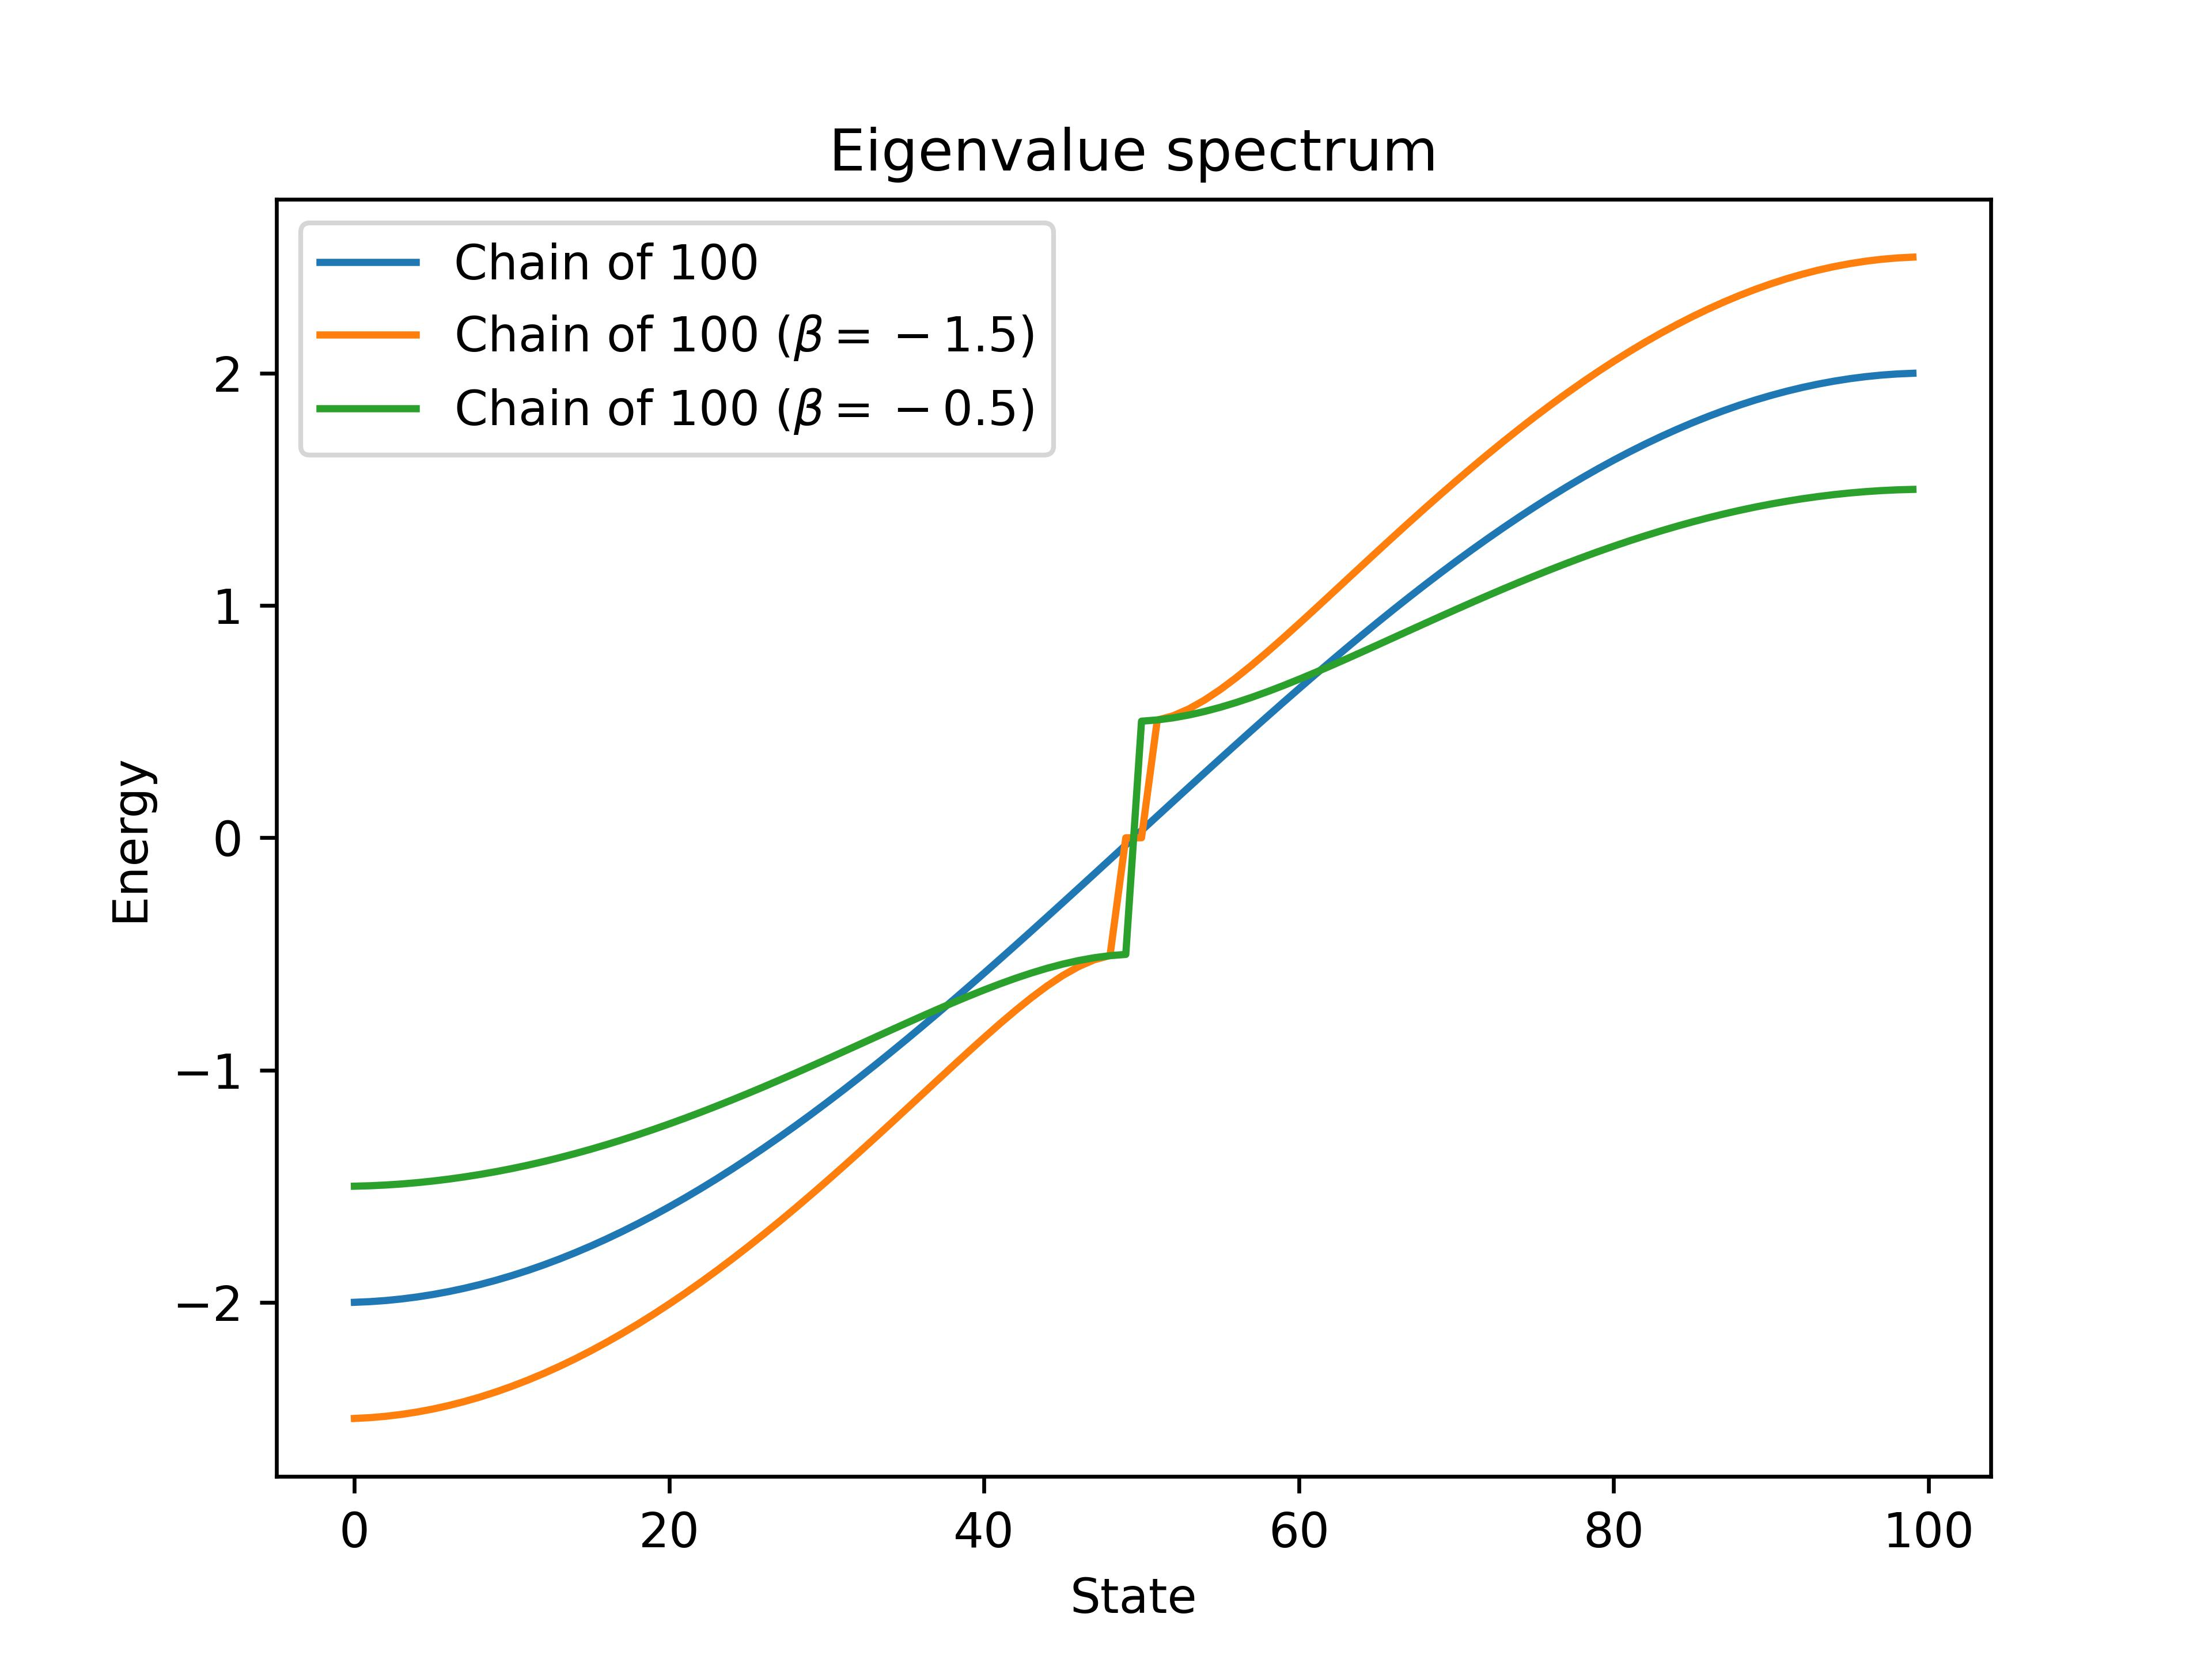
\includegraphics[width=\textwidth]{Figures/chain_beta_eigenvaules.jpg}
        \caption{Eigenvalues for a chain with alternating bond distances.}
        \label{fig:chain_alternating_beta_val}
    \end{minipage}
    \hfill
    \begin{minipage}{0.47\textwidth}
        \centering
        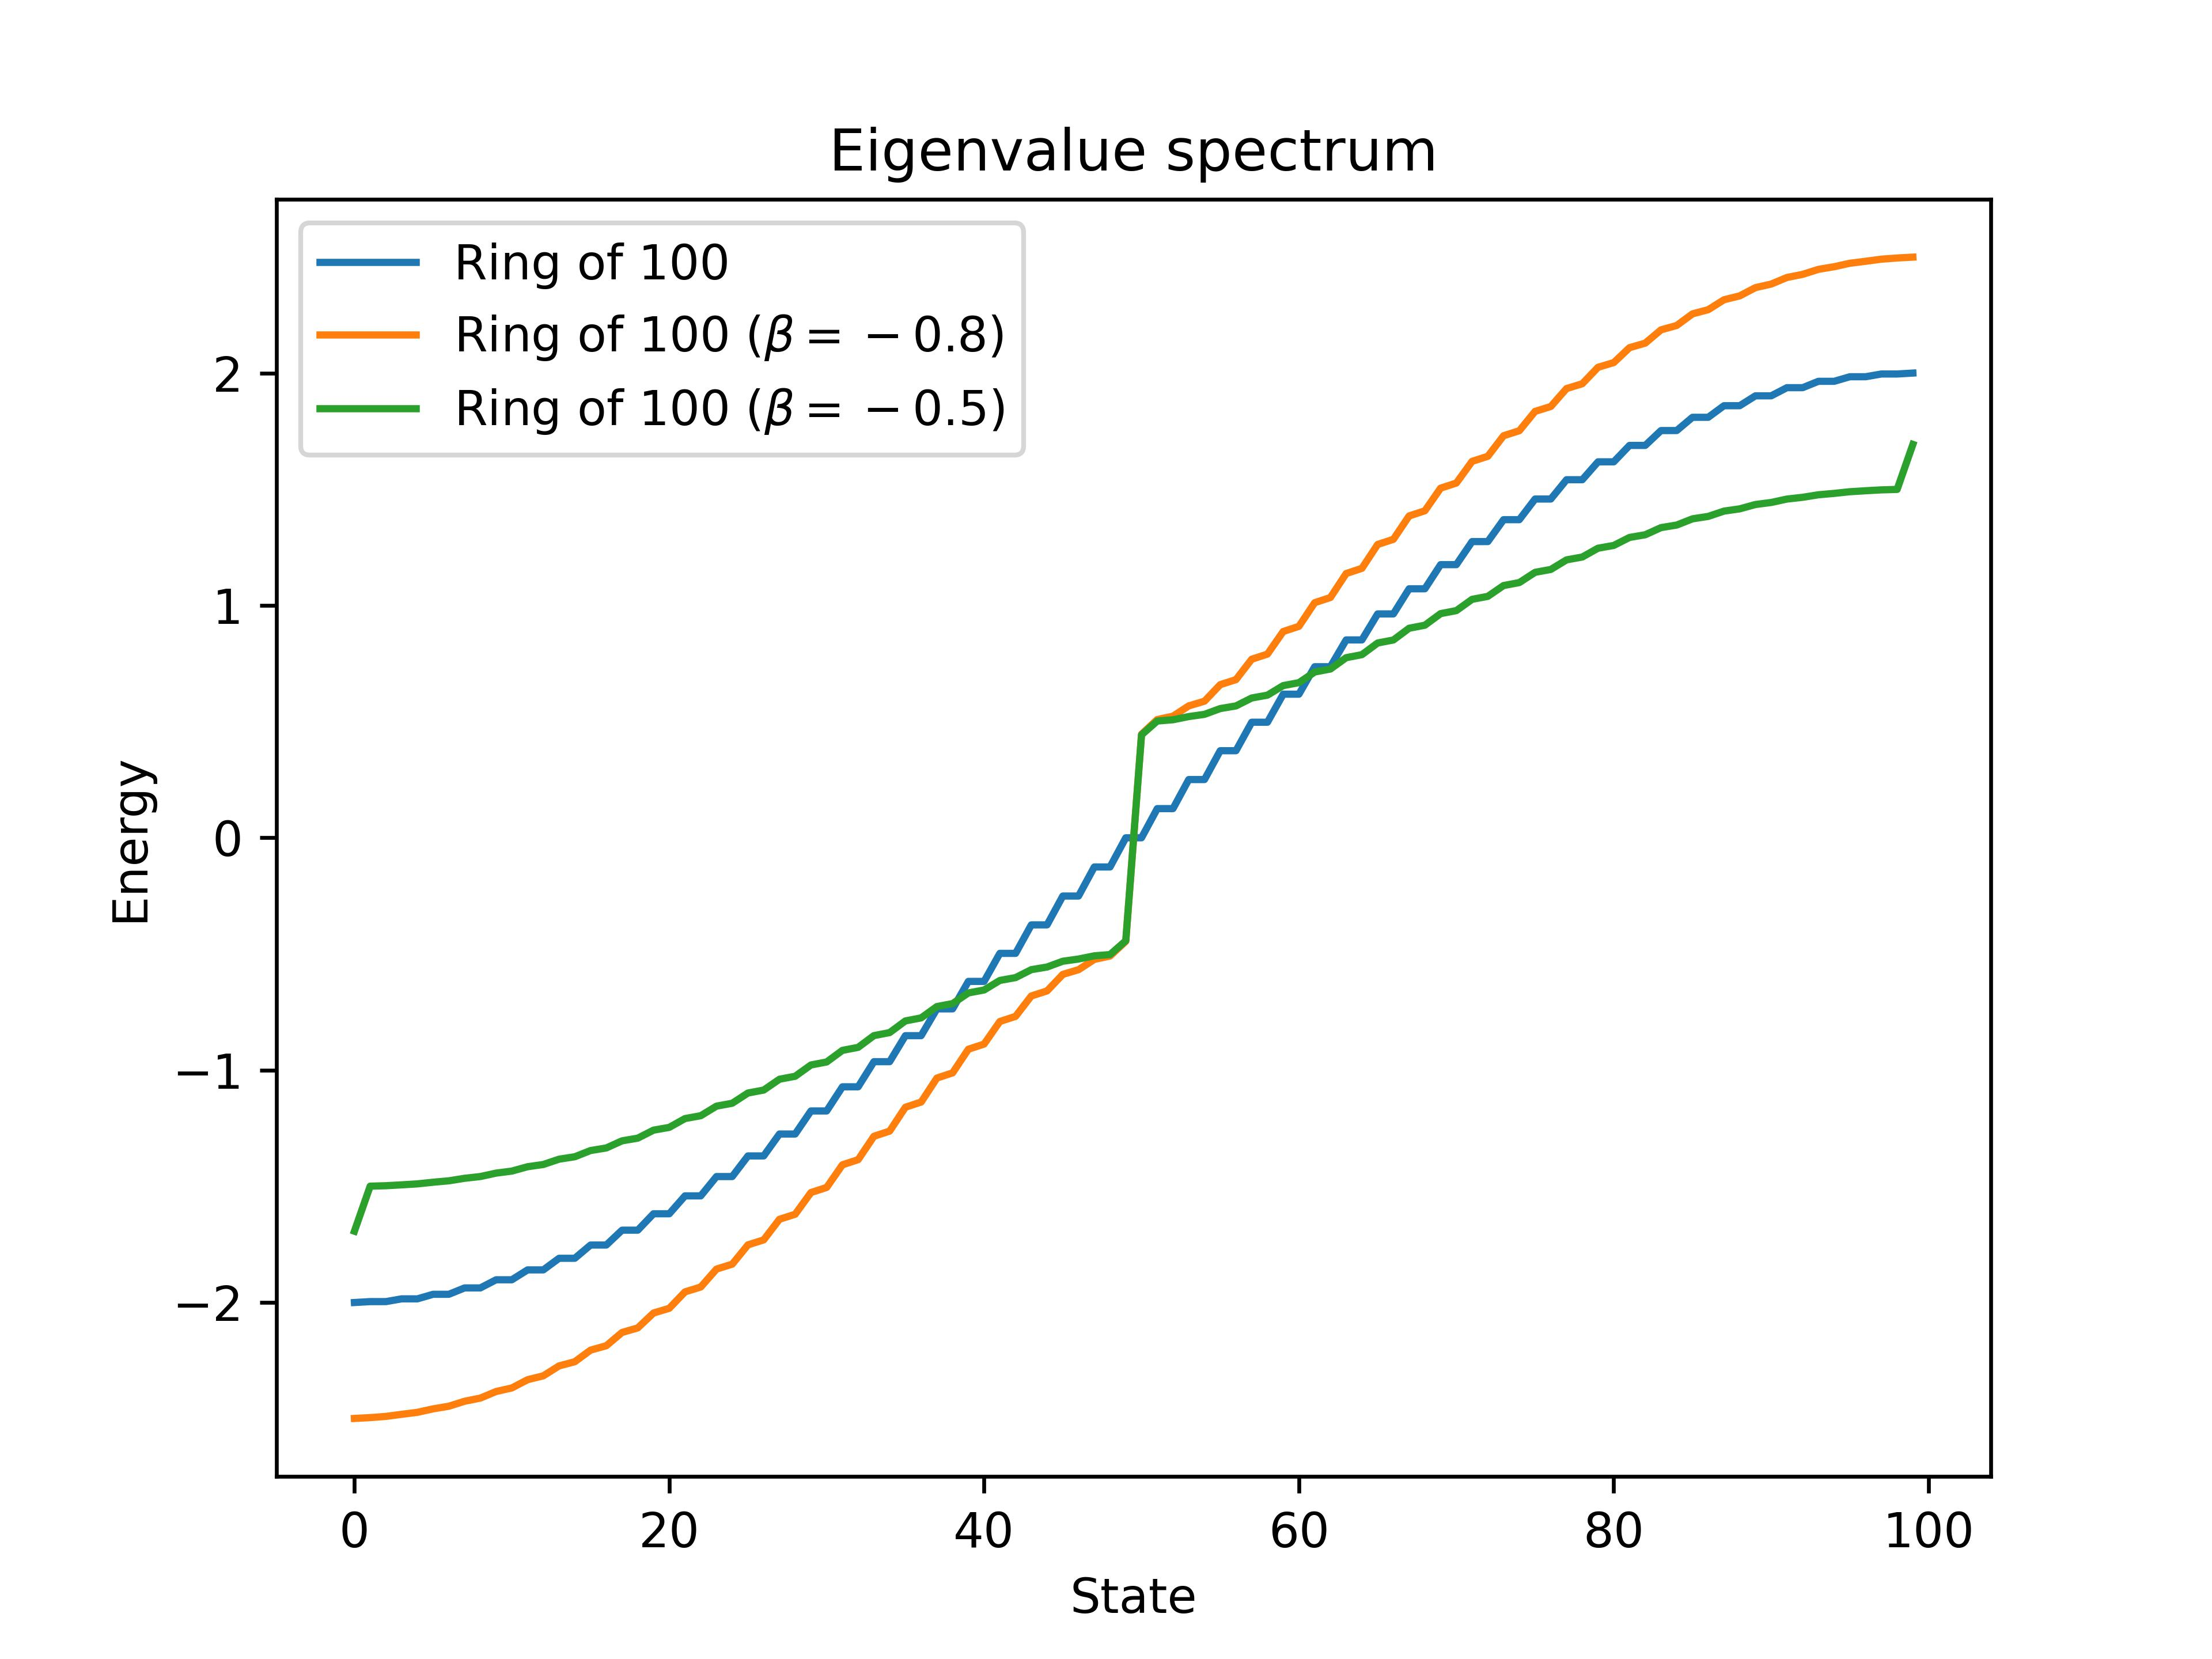
\includegraphics[width=\textwidth]{Figures/ring_beta_eigenvalues.jpg}
        \caption{Eigenvalues for a ring with alternating bond distances.}
        \label{fig:ring_alternating_beta_val}
    \end{minipage}
\end{figure}

The first thing that can be noticed is the difference in the eigenvalues. Both the chain and ring with alternating distances present a new band structure with an energy gap between them centred at $0$. This band gap can be associated with the loss of conjugacy generated by the alternating distances. In the case of the linear or ring systems, the whole conjugated $\pi$-system allows free movement of electrons through the whole system, resulting in a gapless conducting system. Therefore, the differences of distances between neighbours restricts electron movement, resulting in insulation and hence an energy gap between bands. 

On the other hand, the energies of the bands up to the gap differ, with the systems with a smaller (more negative) beta presenting lower valence band energies. This can be explained due to the fact that closer distances will result in stabilizing interactions and thus lower ground state energies. 

Also, due to the loss of conjugacy, the two-fold degeneracy of the ring system is lifted (Figure \ref{fig:ring_alternating_beta_val}), presenting similar eigenvalues for each pair $2n$ and $2n+1$ states, but not exactly the same.

\begin{figure}[ht]
    \centering
    \begin{minipage}{0.47\textwidth}
        \centering
        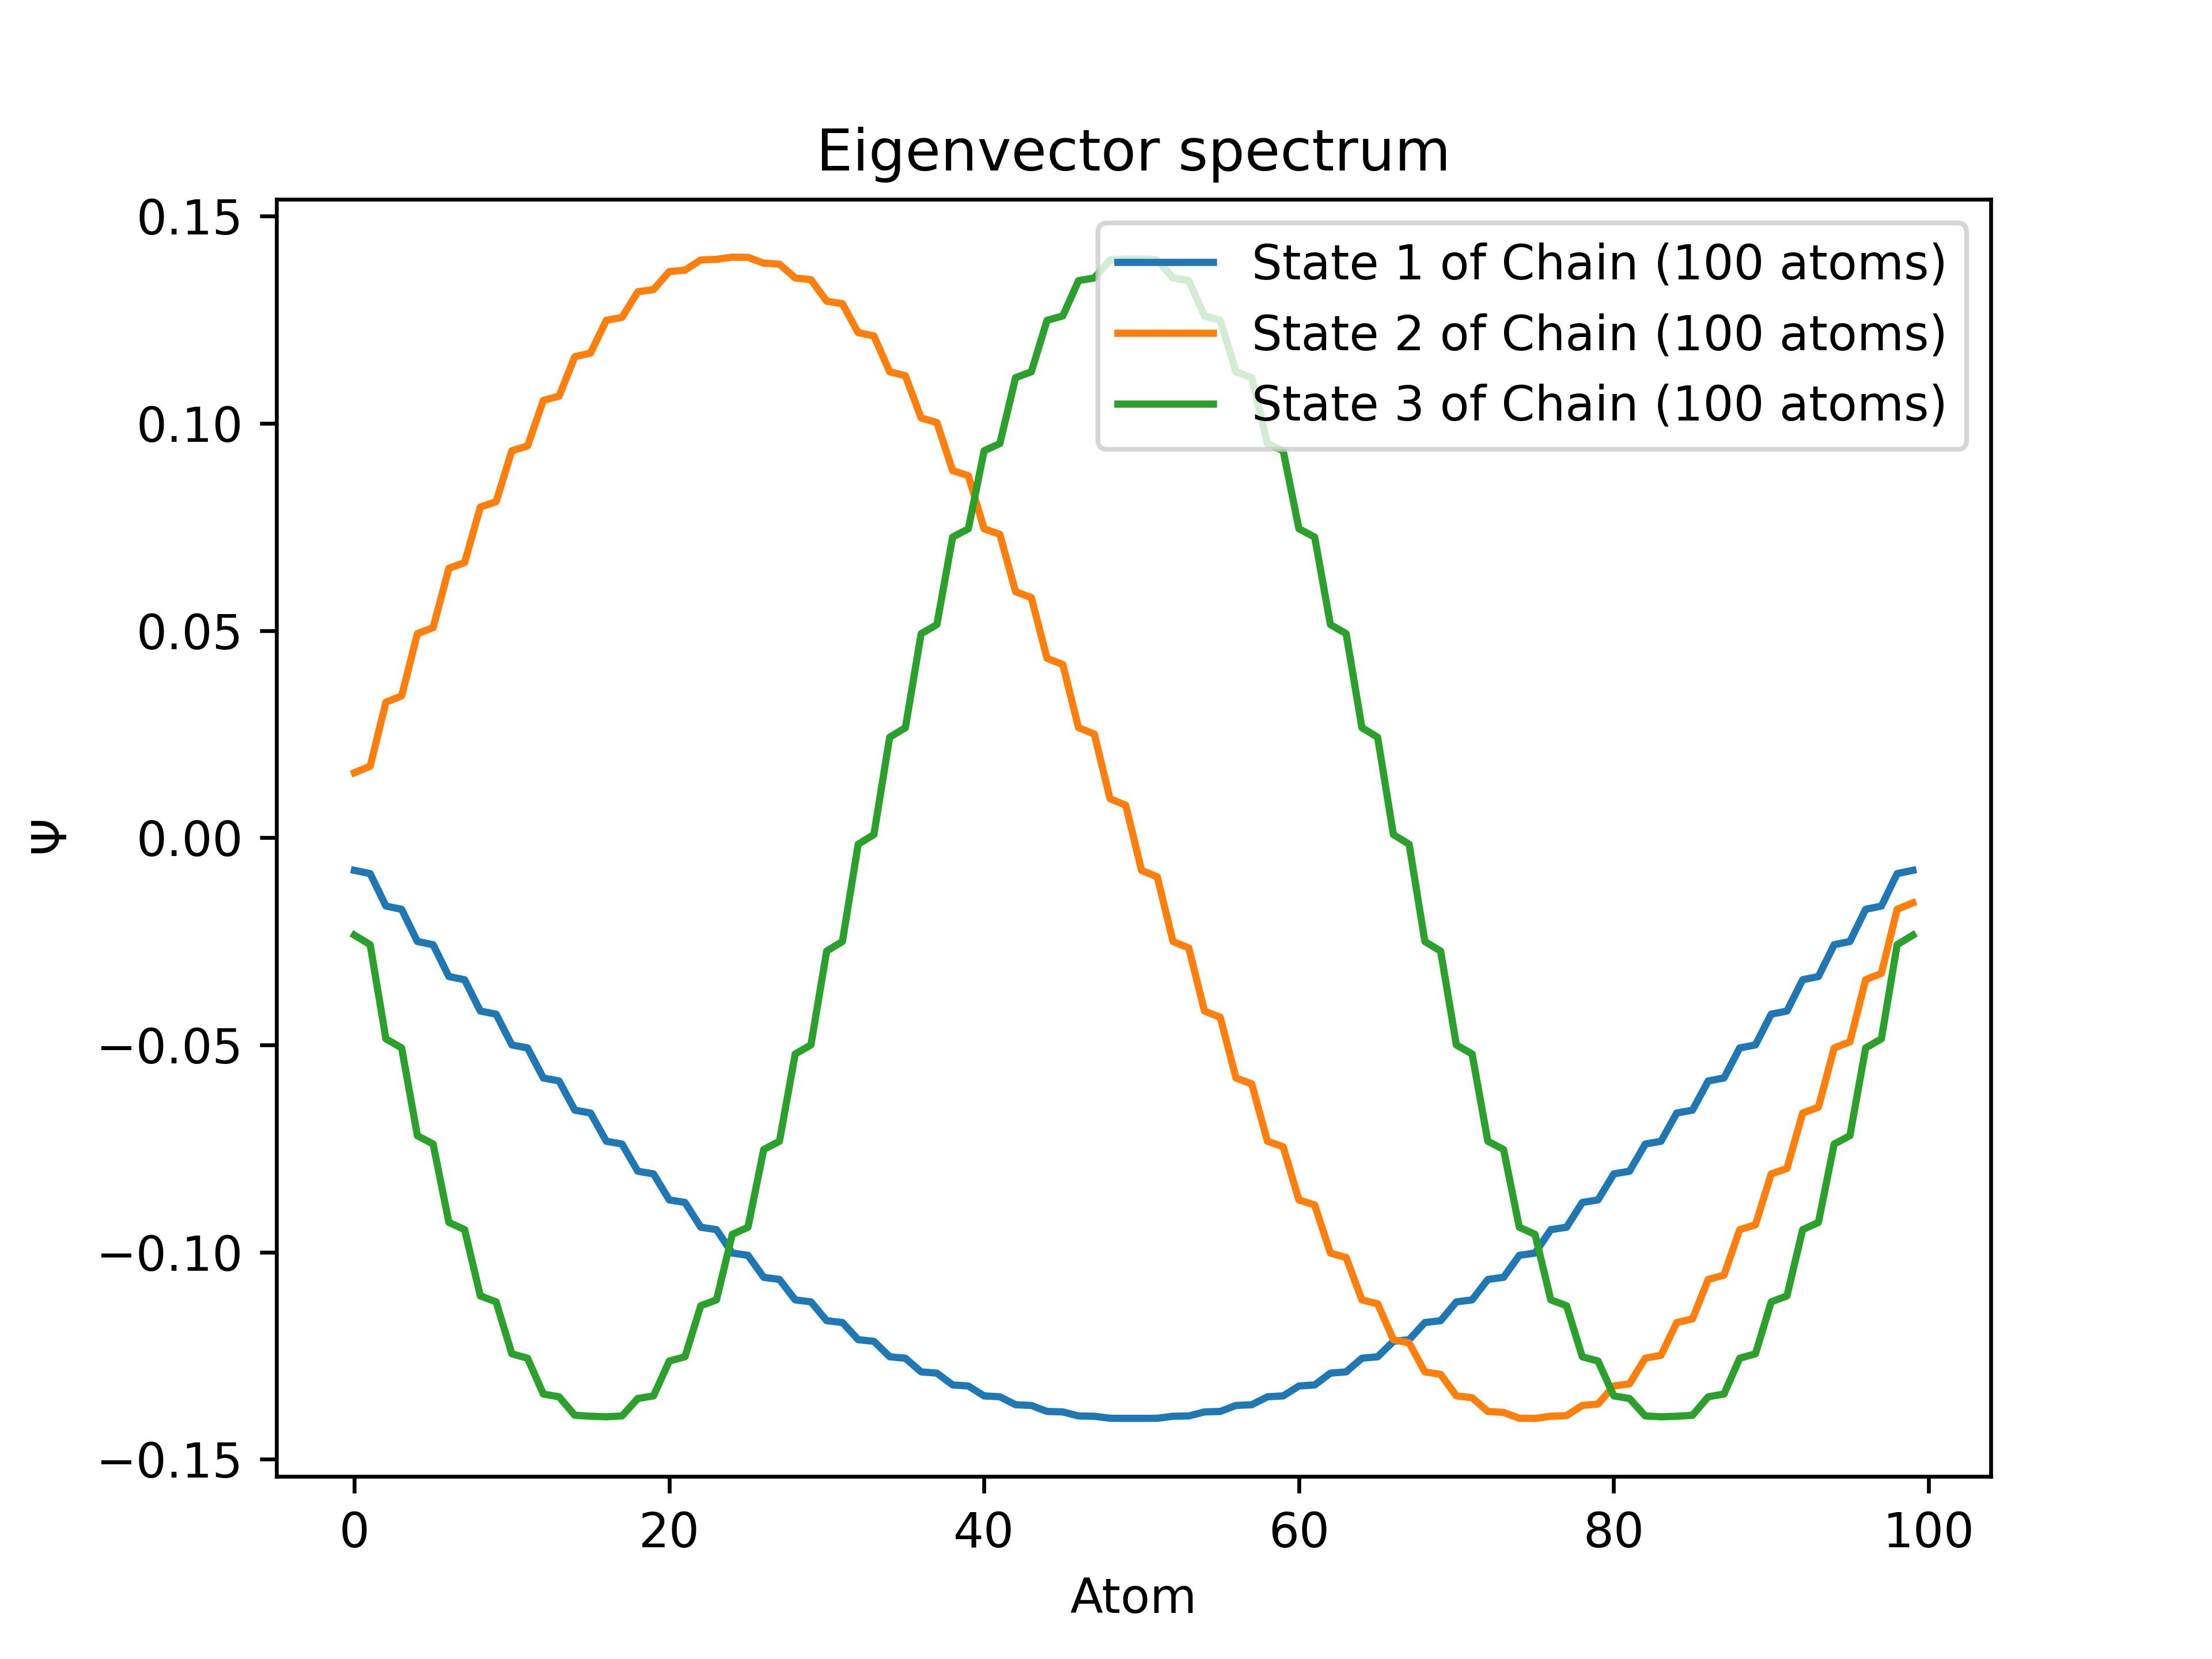
\includegraphics[width=\textwidth]{Figures/beta_chain_eigenvectors.jpg}
        \caption{First states eigenvectors of a chain with alternating bond distances.}
        \label{fig:chain_alternating_beta_vec}
    \end{minipage}
    \hfill
    \begin{minipage}{0.47\textwidth}
        \centering
        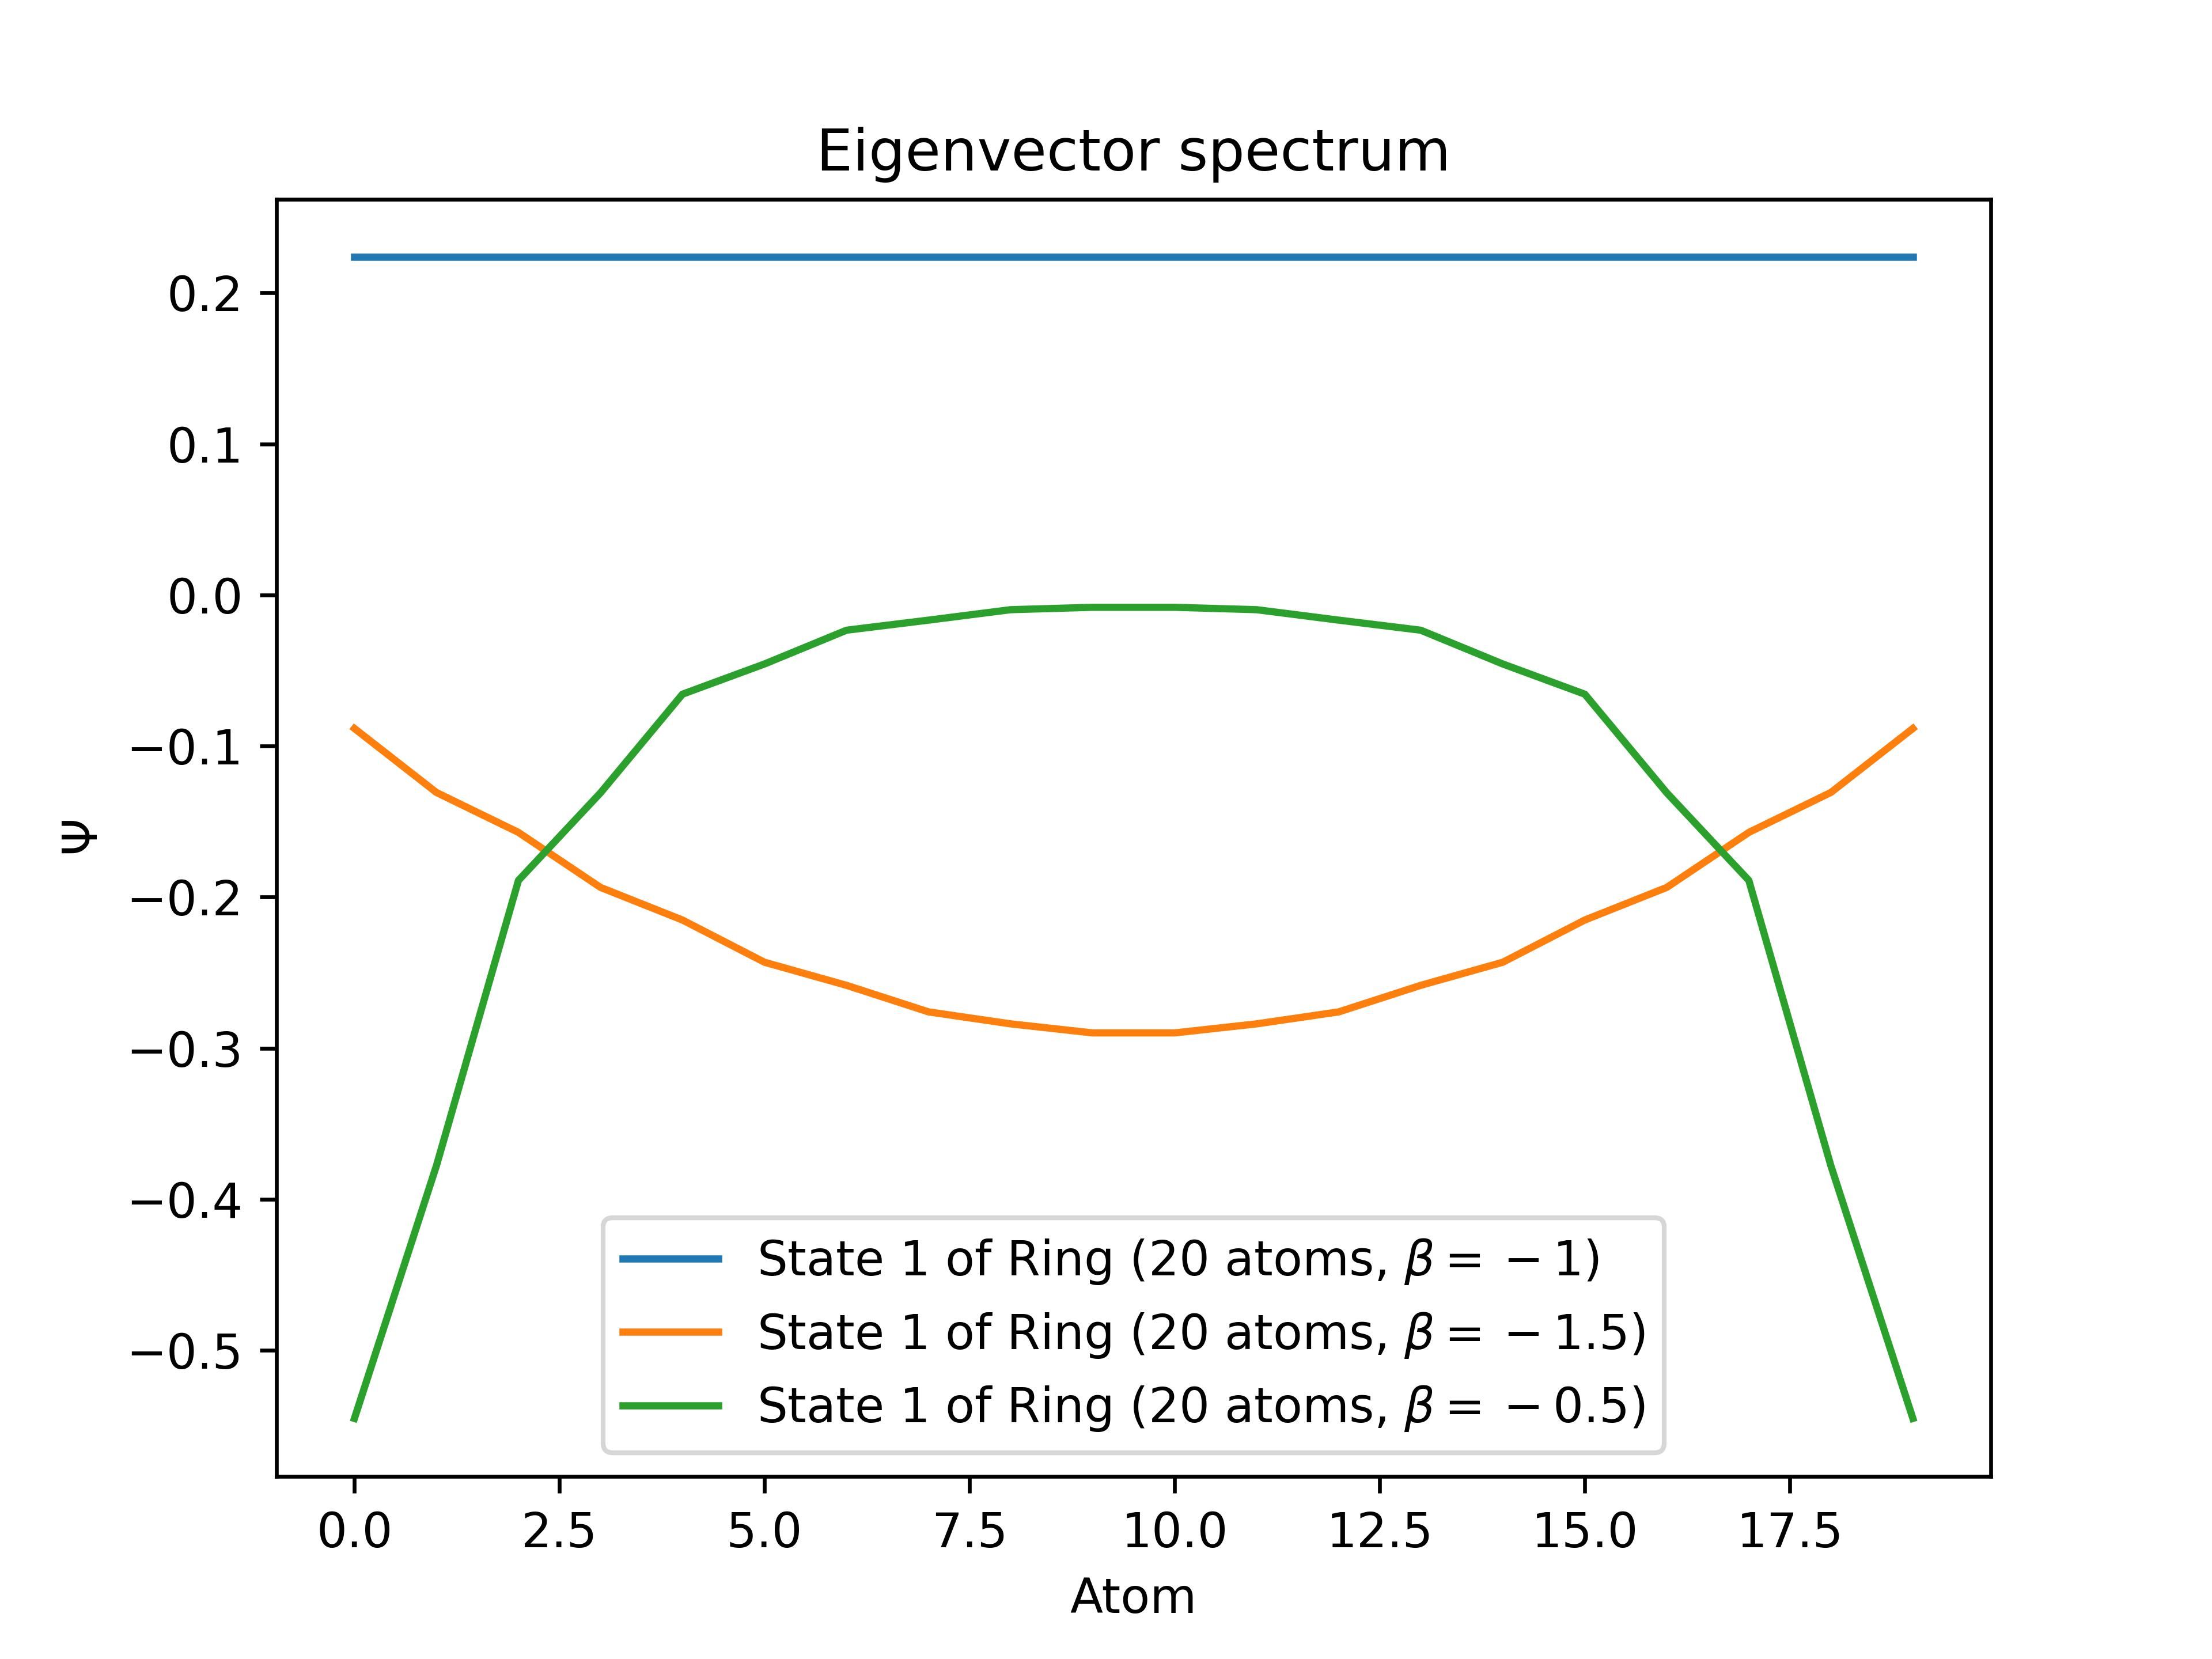
\includegraphics[width=\textwidth]{Figures/ring_beta_eigenvectors.jpg}
        \caption{Ground state eigenvectors of a ring with alternating bond distances.}
        \label{fig:ring_alternating_beta_vec}
    \end{minipage}

\end{figure}

The loss in conjugacy due to alternating atomic distances generates a slight change in the eigenstates of the chain system. What used to be continuous eigenvectors now present a slight pairwise localization in the wave functions (Figure \ref{fig:chain_alternating_beta_vec}). This is explained because due to the different (pairwise) interatomic distances, an electron will be more probable to stay between to closely atoms than to "jump" to an atom much further away. In contrast, the ring wave functions change significantly, being now localized (Figure \ref{fig:ring_alternating_beta_vec}). This localization is extended to the exited states of the system, where the wave functions are not the same but shifted by a phase factor any more. This explains the loss of the two-fold degeneracy of the ring.  Also, the ring eigenstates in this condition behaves similarly to the chain, where the number of nodes in the wave function corresponds to the excited state number.

Mathematically, this whole behaviour can be explained with the Hamiltonian construction and diagonalization. In this case, the diagonal terms are constant, but due to the off-diagonal coupling alternating, this acts as a perturbation on the Hamiltonian, lifting possible degeneracies (in the case of the ring) and generating a gap in the eigenvalue spectrum. Due to the diagonal contribution of alpha, it is possible to separate the Hamiltonian as $H_{eff}^{\alpha\beta} = \mathbb{I} \alpha + H_{eff}^\beta$, which implies that the fermi level will reman at $\alpha$ energy. 

\subsection{Alternating atom types}
The alternating atom types can be simulated with a variation of the $\alpha$ parameter, as each atom type presents a different experimental value. The reference value of alpha has been set to $0$. This implies that a negative value of alpha will result in higher stabilization, while a positive one destabilization. The alternation of $\alpha$ values will result again in the loss of conjugacy. The eigenvalues of the chains and rings are plotted in Figures \ref{fig:chain_alternating_alpha_val} and \ref{fig:ring_alternating_alpha_val}, while eigenvectors in Figures \ref{fig:chain_alternating_alpha_vec} and \ref{fig:ring_alternating_alpha_vec}.

\begin{figure}[ht]
    \centering
    \begin{minipage}{0.47\textwidth}
        \centering
        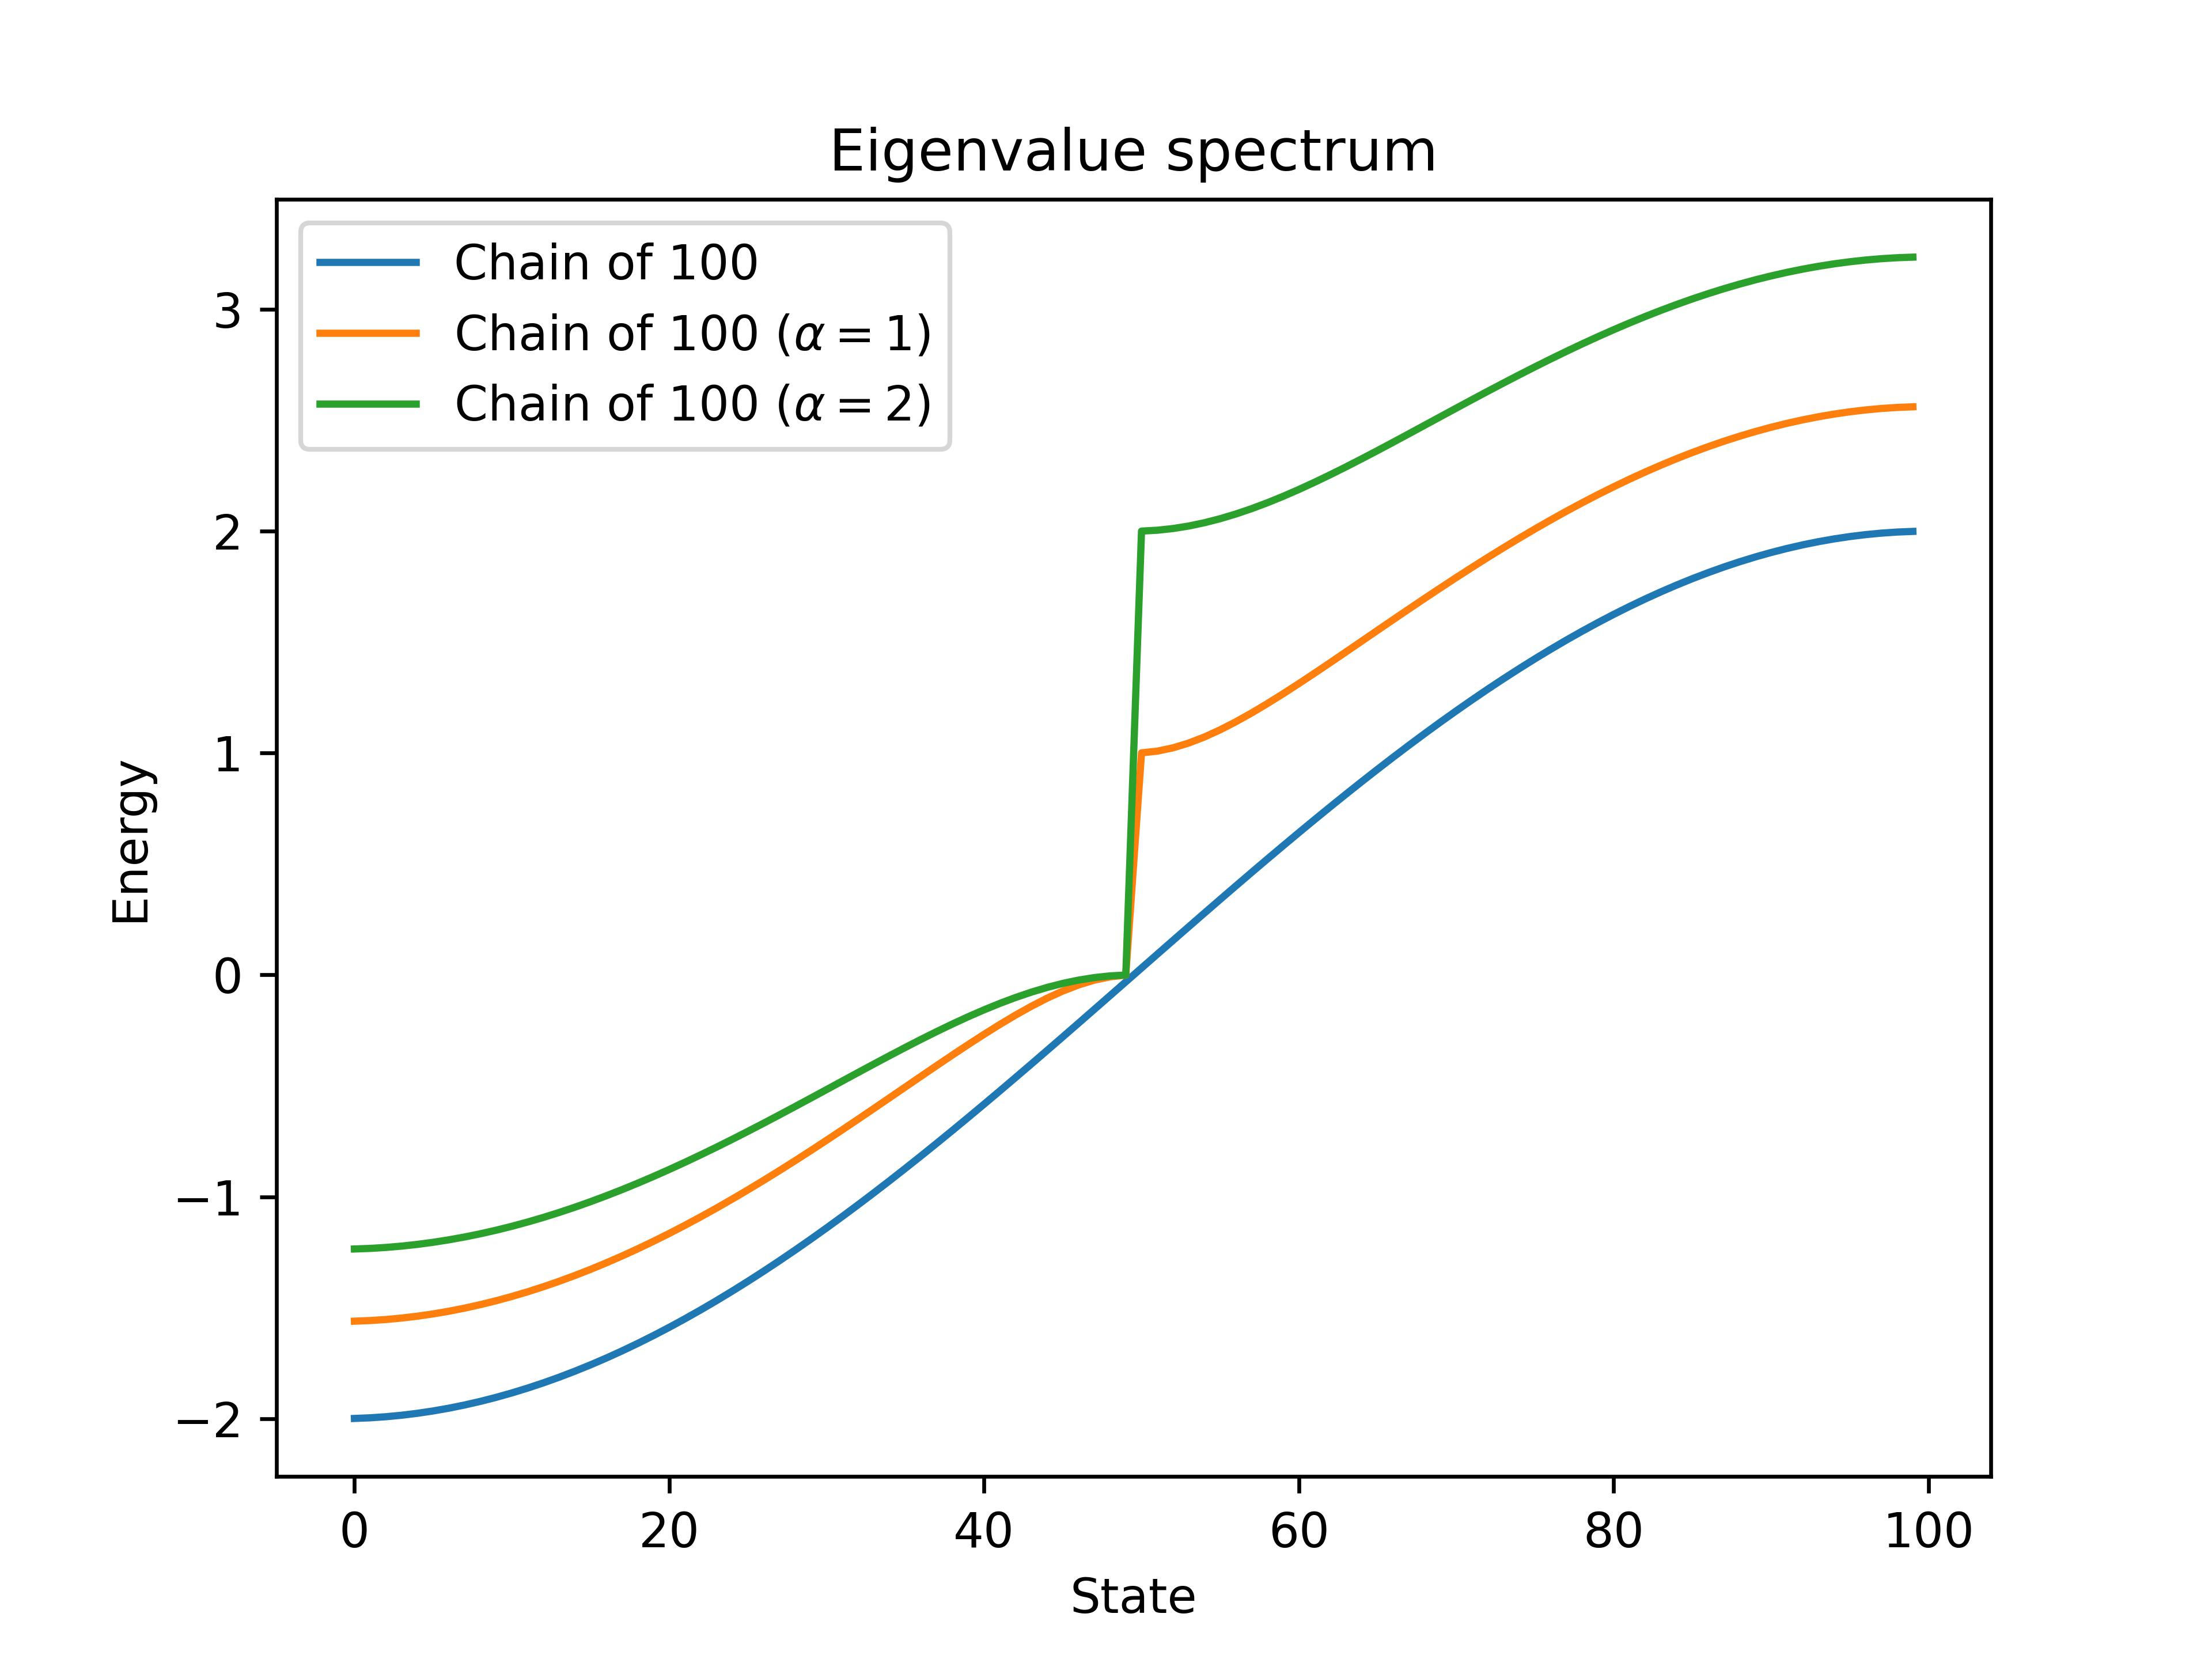
\includegraphics[width=\textwidth]{Figures/alpha_in_chain.jpg}
        \caption{Eigenvalues for a chain with alternating atom types.}
        \label{fig:chain_alternating_alpha_val}
    \end{minipage}
    \hfill
    \begin{minipage}{0.47\textwidth}
        \centering
        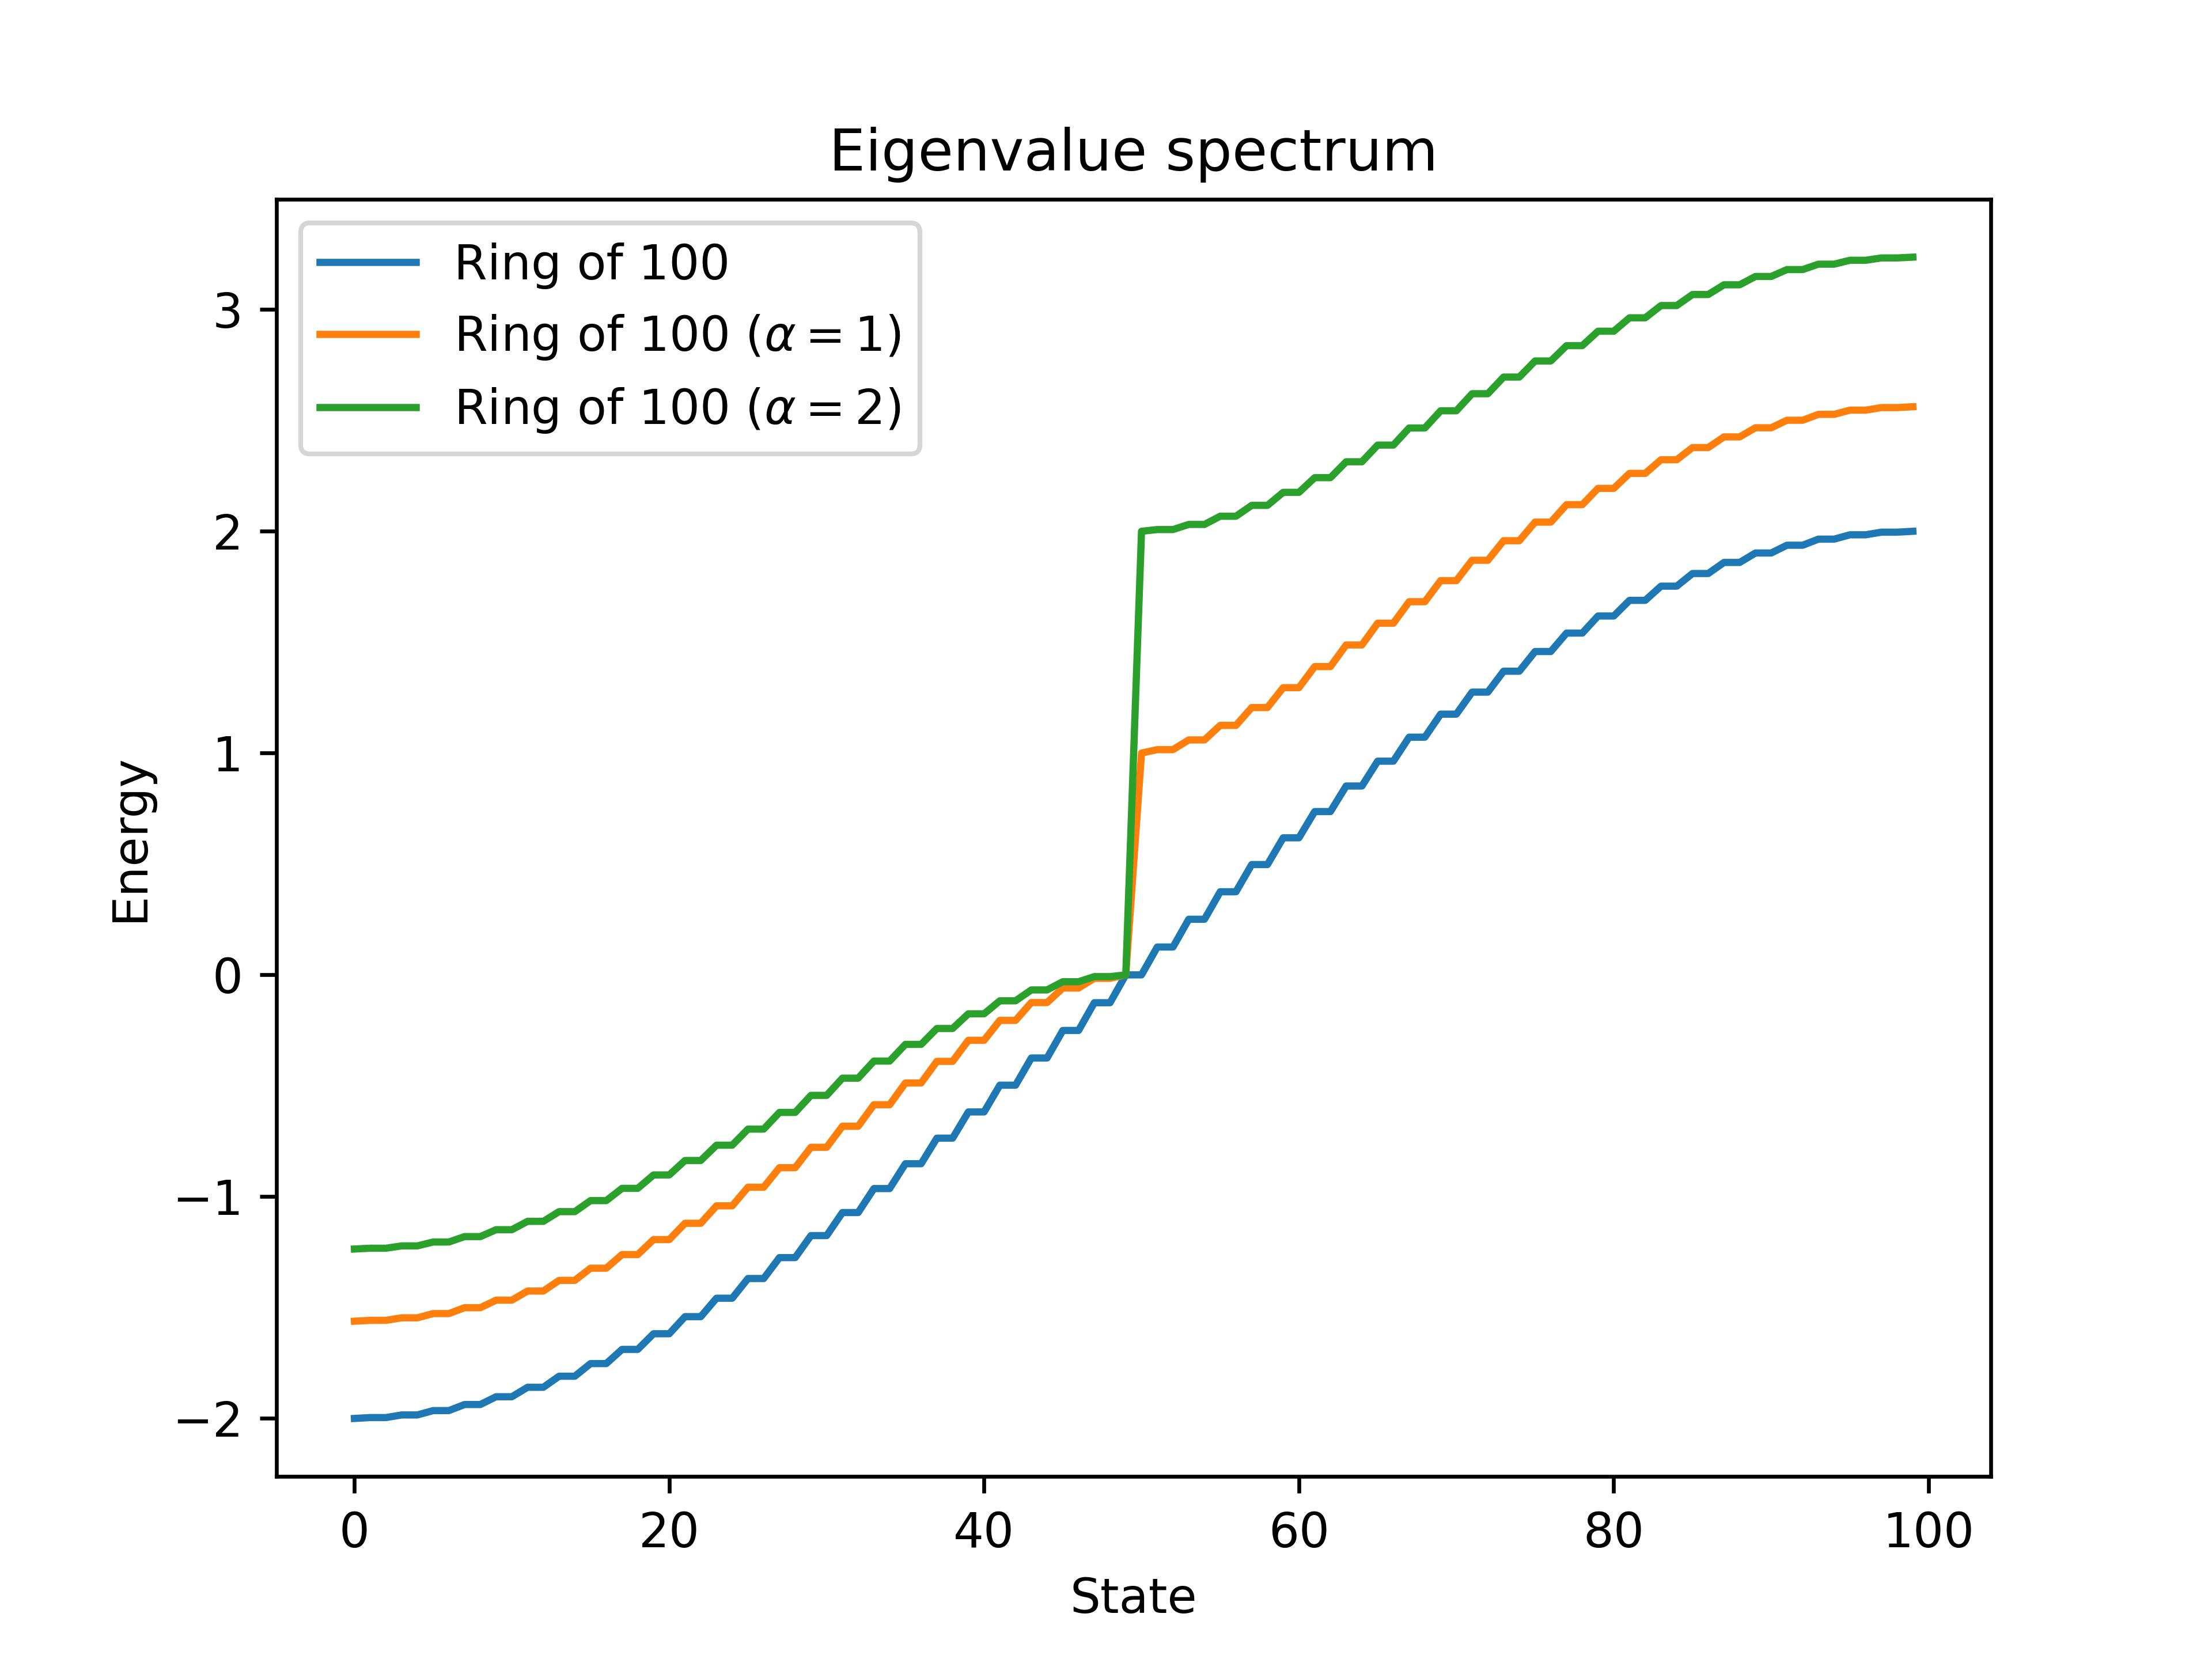
\includegraphics[width=\textwidth]{Figures/alpha_in_ring.jpg}
        \caption{Eigenvalues for a ring with alternating atom types.}
        \label{fig:ring_alternating_alpha_val}
    \end{minipage}
\end{figure}

Again a band gap is found in the energy spectrum, but with a significant change with respect to the previous section, as the Fermi level does not remain at $0$, but is shifted. In Figure \ref{fig:ring_alternating_alpha_val} it is possible that the same value of $\alpha'$ in absolute value results in the same eigenvalue spectrum, but shifted to higher or lower energies depending on the sign. 

This different behaviour can be explained with the Hamiltonian construction. In the base case, the diagonal term is $0$ in all cases, resulting in all eigenvalues being $0 \pm N_i$, the non-diagonal coupling. In the case where the diagonal terms are modified alternating, the eigenvalues can only be  $\alpha-N_i$ or $\alpha'+N_i$ (assuming $\alpha < \alpha'$). This results in the appearance of the gap and the Fermi level being located at $\frac{\alpha + \alpha'}{2}$, shifting the whole eigenvalue spectrum. Also, due to the way the Hamiltonian is constructed in this case, there is no perturbation and therefore the ring eigenvalues will remain two-fold degenerate. 

\begin{figure}[!h]
    \centering
    \begin{minipage}{0.47\textwidth}
        \centering
        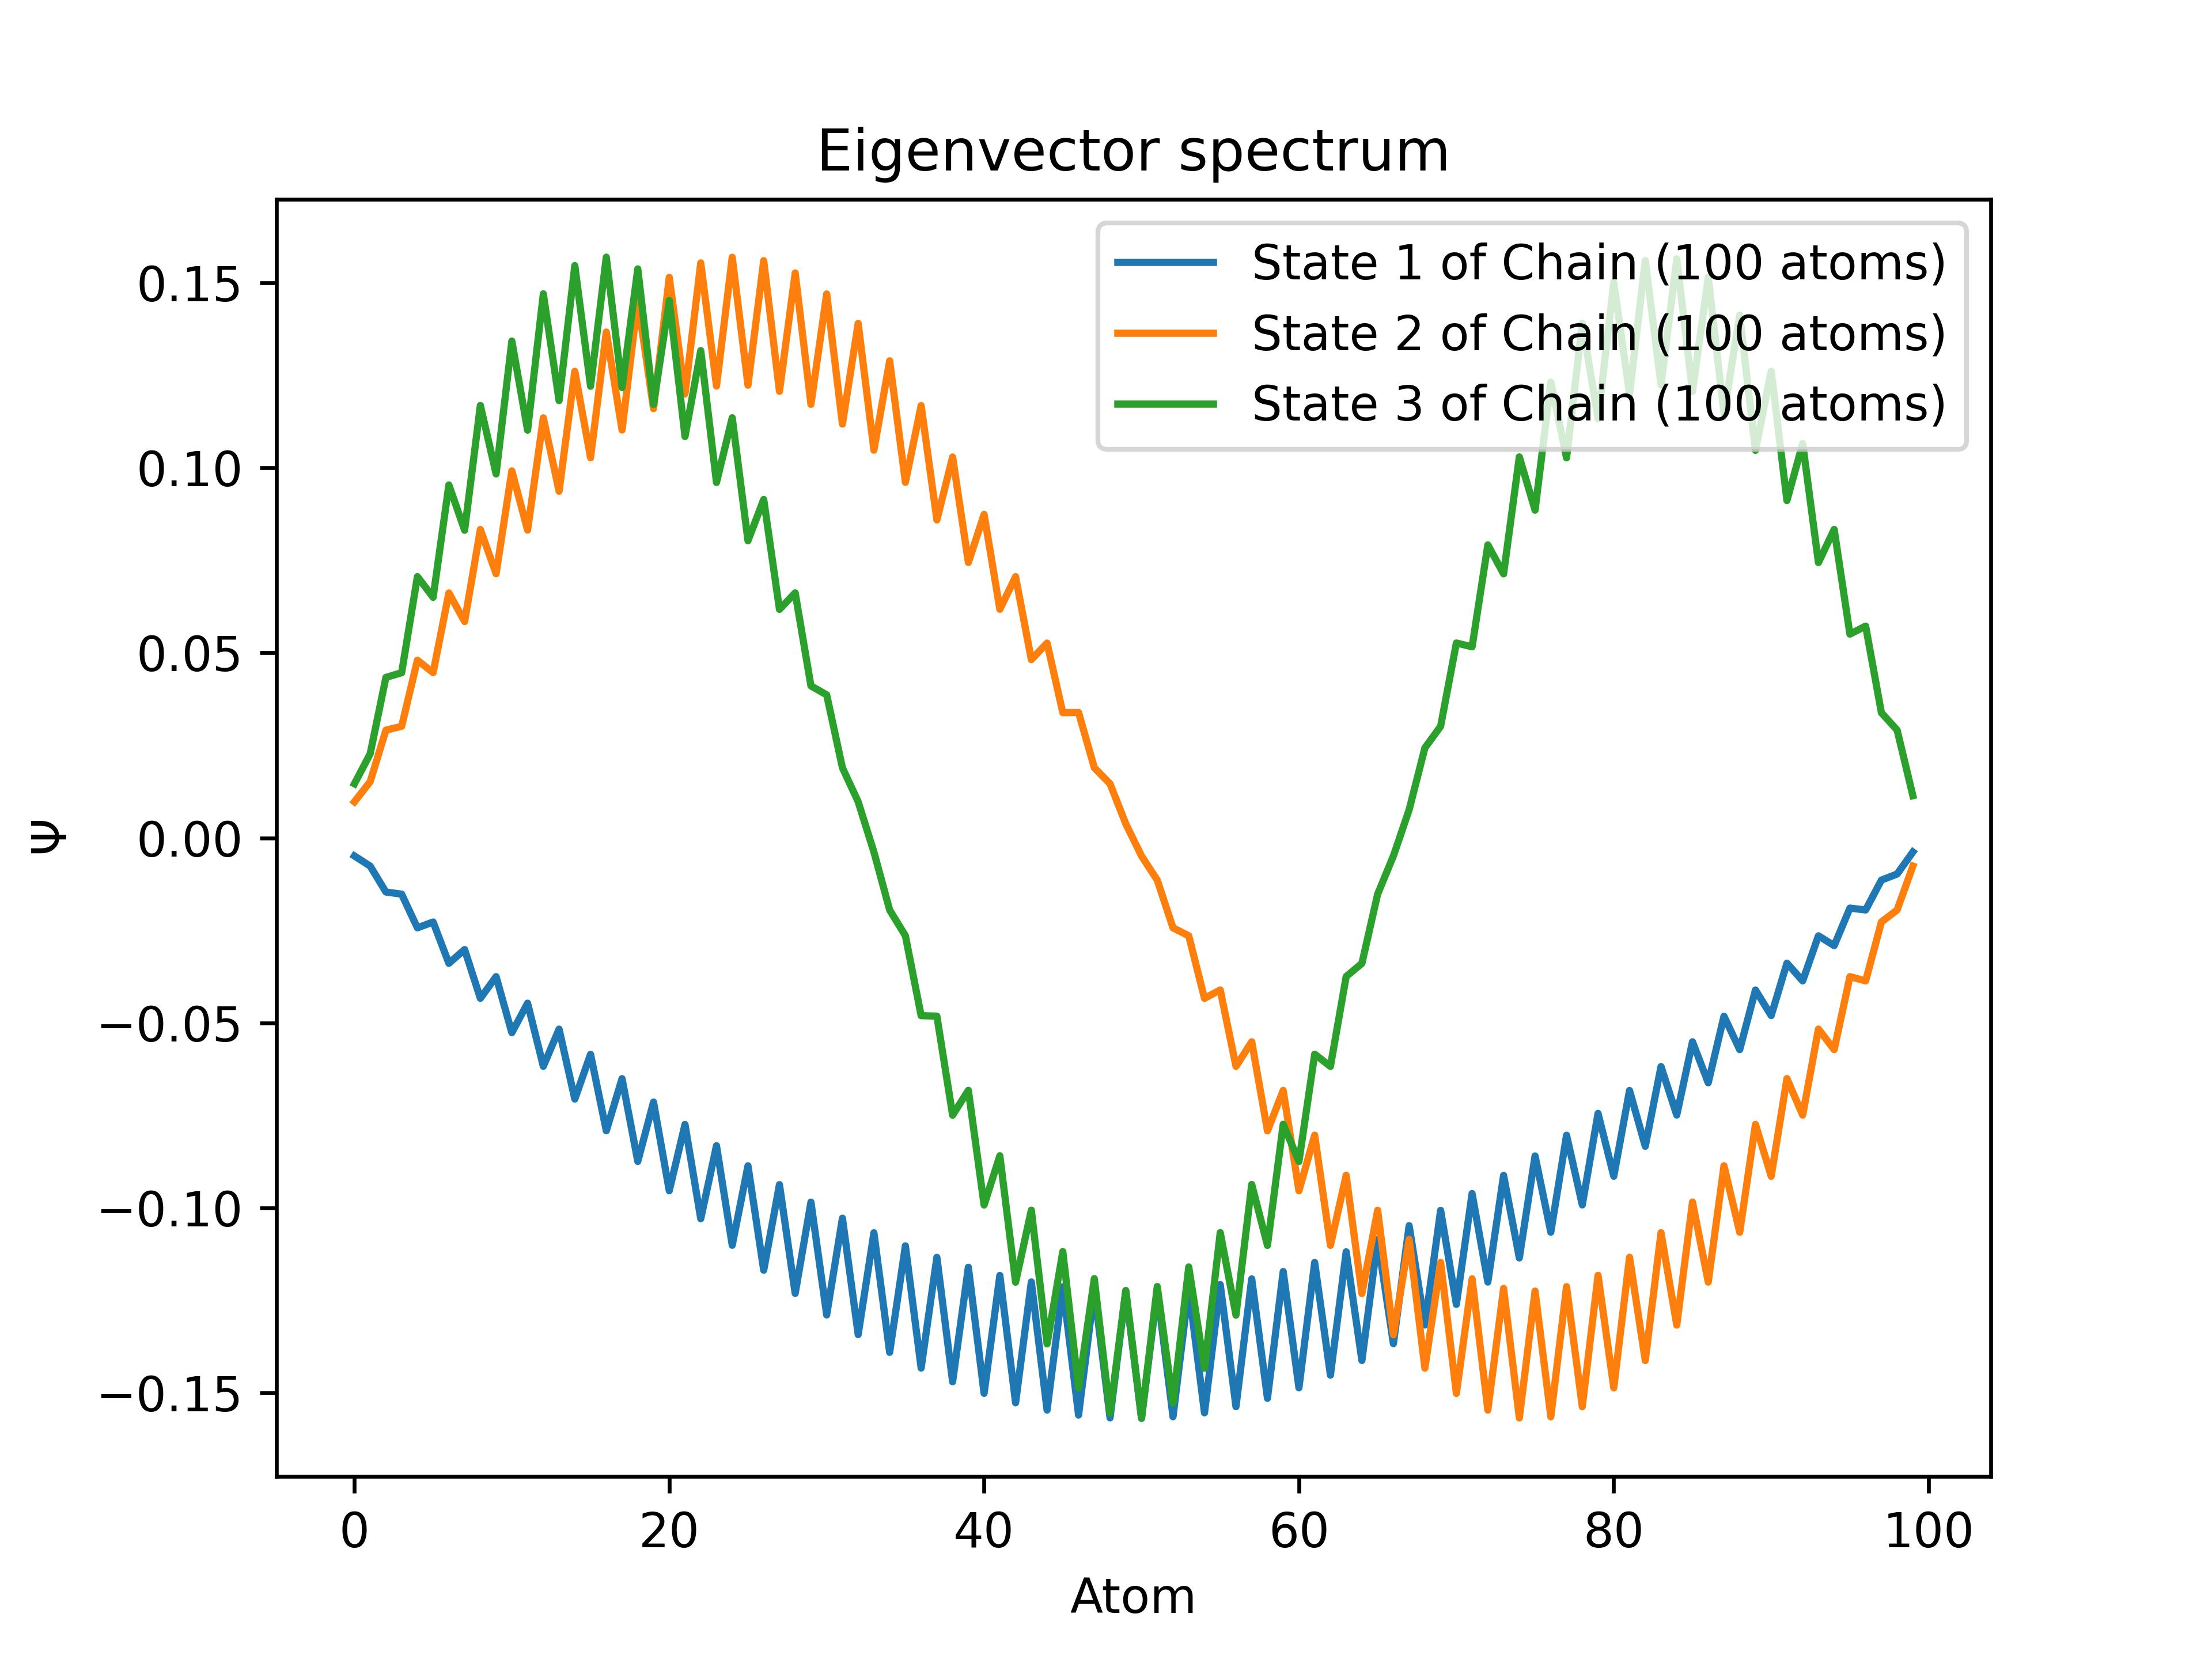
\includegraphics[width=\textwidth]{Figures/chain_alpha_eigenvectors.jpg}
        \caption{Ground state eigenvectors of a chain with alternating atom types.}
        \label{fig:chain_alternating_alpha_vec}
    \end{minipage}
    \hfill
    \begin{minipage}{0.47\textwidth}
        \centering
        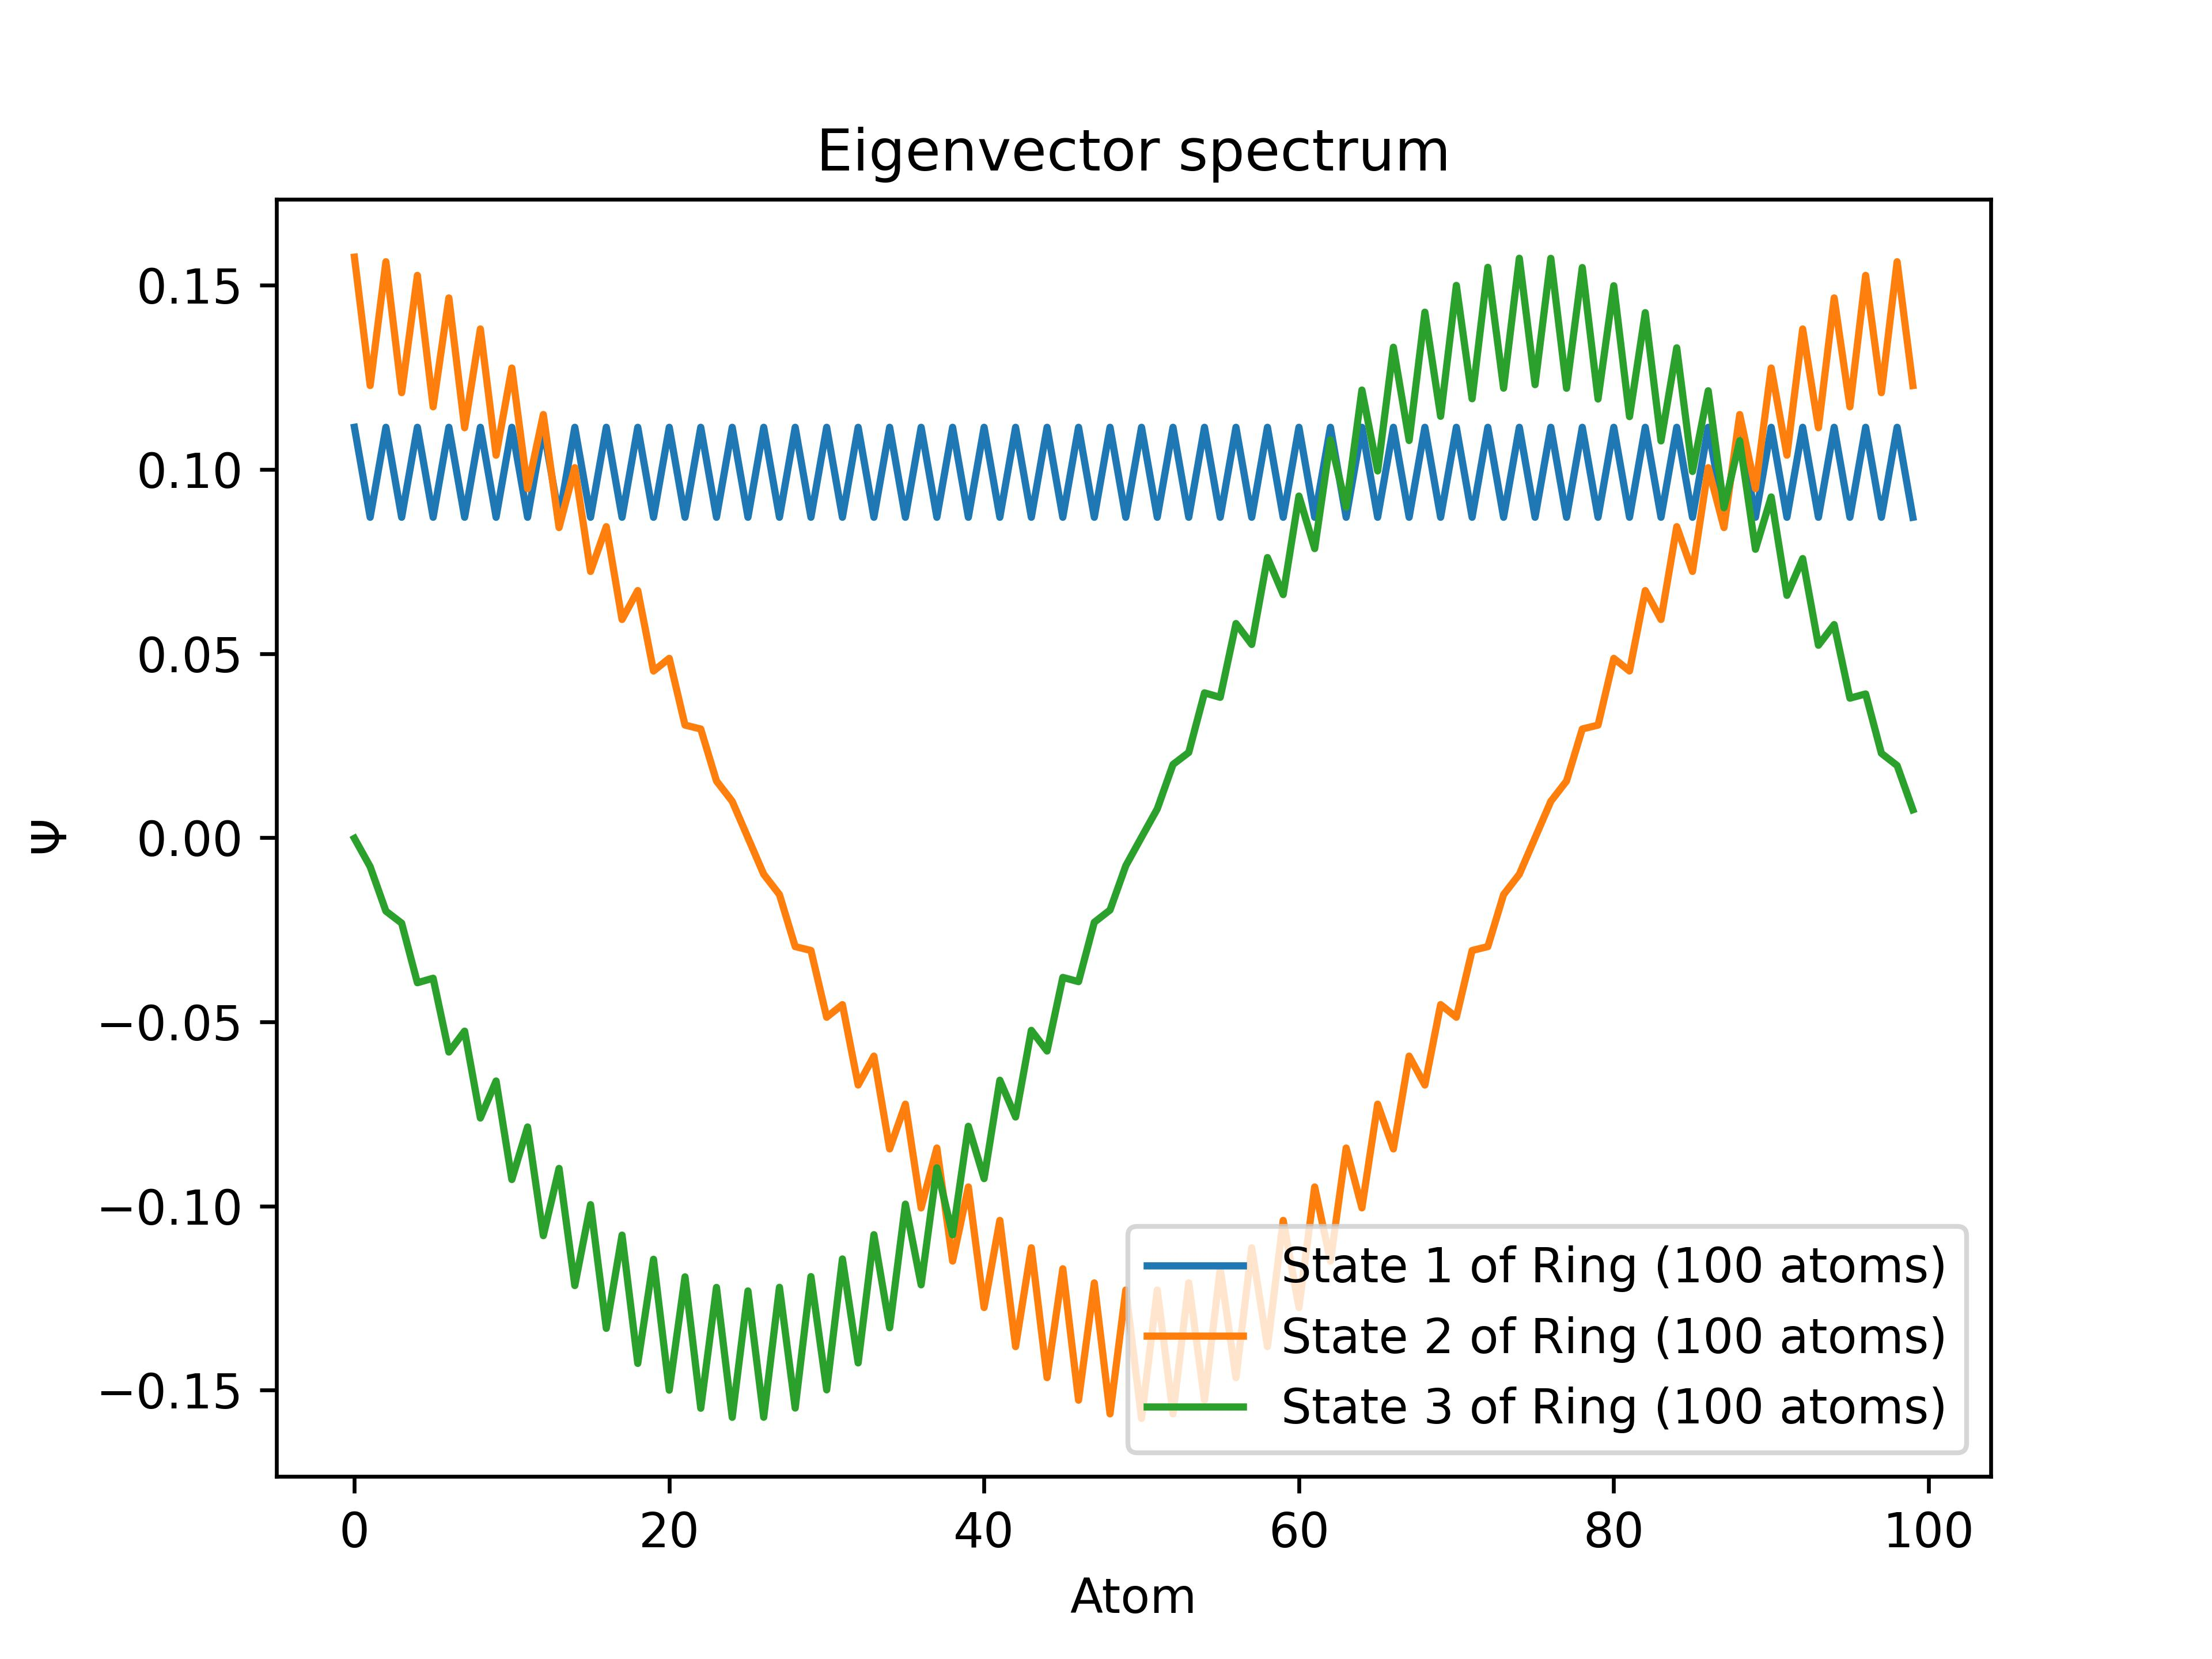
\includegraphics[width=\textwidth]{Figures/ring_alpha_eigenvectors.jpg}
        \caption{Ground state eigenvectors of a ring with alternating atom types.}
        \label{fig:ring_alternating_alpha_vec}
    \end{minipage}
\end{figure}

The eigenvector spectrum is identical in shape to the base case, with the exception that there is an oscillation in probability between alternating atoms. This is due to the relative difference in binding energy between the different atoms, where the probability of being bound to an atom will increase if the binding energy is lower. 

\section{Conclusions}
In this report, a program to calculate the eigenvalues and eigenvectors of the Hückel Hamiltonian for carbon chains and rings was implemented. The program allows for the simulation of different scenarios, including alternating bond distances and alternating atom types. All the results are in agreement with Hückel MO theory, implying a correct implementation in the program. 

Chains and rings were proven to exhibit different eigenvalues and eigenvector spectra, with rings showing two-fold degeneracy due to PBC. The behaviour of both was proven to converge at the infinite length limit. 

Due to the nature of the Hamiltonian, a change in either bond distances or bond types result in a loss of conjugacy and therefore the appearance of a gap in the band structure. A change in distances results in the modification of the eigenvalue spectrum generating a symmetric band gap centred around the zero energy level and breaking degeneracy in the ring. In contrast, the modification of atom types not only generates a band gap, but shifts the energy of the fermi level while maintaining the degeneracy in the ring. 

The wave function is also modified by these changes. Different atomic distances results in a wave function localization within the chain or ring structure, and thus a loss of degeneracy in the ring, whereas a change in atom types results in localization on certain atoms, maintaining degenerate states in the ring system.      

\printbibliography

\end{document}

